\documentclass[thesis=M,czech]{FITthesis}[2019/12/23]

\usepackage{xevlna}
\usepackage{minted}
\usemintedstyle{manni}
\makeatletter\AtBeginDocument{\let\@elt\relax}\makeatother
\AtBeginDocument{\counterwithin{listing}{chapter}}

\usepackage[utf8]{inputenc} % LaTeX source encoded as UTF-8

\usepackage{amsmath} %advanced maths
\usepackage{amssymb} %additional math symbols

\usepackage{graphicx}
\graphicspath{ {./img/} }

\usepackage{dirtree} %directory tree visualisation
\RequirePackage{pdfpages}

% % list of acronyms
% \usepackage[acronym,nonumberlist,toc,numberedsection=autolabel]{glossaries}
% \iflanguage{czech}{\renewcommand*{\acronymname}{Seznam pou{\v z}it{\' y}ch zkratek}}{}
% \makeglossaries

\newcommand{\tg}{\mathop{\mathrm{tg}}} %cesky tangens
\newcommand{\cotg}{\mathop{\mathrm{cotg}}} %cesky cotangens

% % % % % % % % % % % % % % % % % % % % % % % % % % % % % % 
% ODTUD DAL VSE ZMENTE
% % % % % % % % % % % % % % % % % % % % % % % % % % % % % % 

\department{Katedra softwarového inženýrství}
\title{Srovnání REST, GraphQL a gRPC API v~Node.js}
\authorGN{Tomáš} %(křestní) jméno (jména) autora
\authorFN{Buňata} %příjmení autora
\authorWithDegrees{Bc. Tomáš Buňata} %jméno autora včetně současných akademických titulů
\author{Tomáš Buňata} %jméno autora bez akademických titulů
\supervisor{Ing. Lukáš Loukota}
\acknowledgements{Na tomto místě bych rád poděkoval všem lidem, kteří mi pomáhali při vzniku této práce. V prvé řadě Lukáši Loukotovi, vedoucímu mé diplomové práce, za cenné podněty k textové části i implementacím. Dále bych rád poděkoval svojí rodině a přátelům za důvěru a podporu.}
\abstractCS{Tato diplomová práce si klade za cíl srovnání tří technologií pro tvorbu API -- REST, GraphQL a gRPC. V první části práce jsou tyto technologie nejdříve představeny společně s výběrem populárních knihoven vhodných k jejich implementaci. Poté je představen návrh API, který je následně implementován v každé z těchto technologií. Poslední část práce se věnuje zátěžovým testům a srovnání z pohledu výkonu, dokumentace nebo developer experience.}
\abstractEN{This master's thesis aims to compare three technologies for creating an API -- REST, GraphQL, and gRPC. The first part of this thesis introduces those technologies together with an overview of popular libraries suited for implementation. The next part focuses on the design and implementation of API in each of those technologies. The implementations are then compared from the points of performance, documentation, or developer experience.}
\placeForDeclarationOfAuthenticity{V~Praze}
\declarationOfAuthenticityOption{4} %volba Prohlášení (číslo 1-6)
\keywordsCS{web, API, REST, GraphQL, gRPC, Node.js, TypeScript}
\keywordsEN{web, API, REST, GraphQL, gRPC, Node.js, TypeScript}
% \website{http://site.example/thesis} %volitelná URL práce, objeví se v tiráži - úplně odstraňte, nemáte-li URL práce

\begin{document}

% \newacronym{CVUT}{{\v C}VUT}{{\v C}esk{\' e} vysok{\' e} u{\v c}en{\' i} technick{\' e} v Praze}
% \newacronym{FIT}{FIT}{Fakulta informa{\v c}n{\' i}ch technologi{\' i}}

\begin{introduction}
Webové aplikace jsou každodenní součástí našeho života. Setkáváme se s nimi při čtení ranních zpráv, komunikaci se svými přáteli nebo spravování financí přes internetové bankovnictví.

Architektura webových aplikací se dá rozdělit na dvě hlavní části: frontend (část se kterou interaguje uživatel v prohlížeči) a backend (serverová část, která slouží k ukládání a manipulaci s daty). V této práci se věnuji té druhé části -- konkrétně backendovým technologiím zprostředkovávající komunikaci mezi serverem a klientem.

Vzhledem k tomu, že webové technologie se velmi rychle vyvíjejí a posouvají vpřed, vývojáři velmi často narážejí na otázku výběru správné technologie pro svůj projekt. V této práci se pokusím na tuto otázku odpovědět. Porovnám mezi sebou následující: REST, GraphQL a gRPC.

V roce 2000 byl vynalezen REST, který je z těchto technologií nejstarší a v současnosti také nejpopulárnější. Princip RESTu je takový, že každá entita je identifikována unikátním URI a pomocí HTTP metod je s těmito entitami manipulováno.
GraphQL vzniklo přibližně o deset let později a funguje zcela na odlišném principu -- vystavuje jediný endpoint, na který se poté dotazujeme speciálním jazykem, který strukturou velmi připomíná JSON.
Nejmladší z těchto technologií je gRPC, které vzniklo v roce 2015, a jedná se o open source implementaci RPC (volání vzdálené procedury) od společnosti Google.

S každou z těchto technologií implementuji aplikační rozhraní pro e-shop a následně je porovnám ze stránek výkonu, zkušenosti s vývojem nebo dokumentace API.
V teoretické části práce nejdříve tyto technologie představím. Následně uvedu knihovny, které se často používají k implementaci jednotlivých API. Poté se budu věnovat požadavkům na návrh backendu aplikace, na kterém tyto technologie budou demonstrovány.
V praktické části se budu nejdříve věnovat implementaci jednotlivých backendů, včetně otestování jejich správné funkčnosti, a poté otestuji jejich výkon zátěžovými testy. Poslední část se bude věnovat samotnému srovnání těchto technologií.

\end{introduction}

\chapter{Analýza}
Před tím, než se začnu věnovat návrhu a implementaci API, je důležité nejdříve vysvětlit, co tento pojem znamená a následně představím samotné technologie REST, GraphQL a gRPC.

\section{Aplication programming interface}
Zkratka API označuje rozhraní pro programování aplikací. Jedná se o velmi důležitou součást vývoje, protože definuje způsob, jak mezi sebou budou jednotlivé aplikace (nebo komponenty v rámci jedné aplikace) komunikovat. Dalo by se říci, že představuje smlouvu, kterou obě strany musí dodržet, aby spolu mohly komunikovat.

API se skládá ze dvou částí: 
\begin{itemize}
    \item Technické specifikace, která popisuje možnosti komunikace -- metody, které API vystavuje, vstupní data atd.
    \item Softwarového rozhraní, které tuto specifikaci implementuje
\end{itemize}

API se dále mohou dělit podle dostupnosti na soukromá, partnerská nebo otevřená. 

Soukromá API se používají výhradně v rámci jedné organizace. I když aplikace, které tato API využívají mohou být veřejně dostupné, samotné rozhraní není.

Partnerská API jsou sdílená s business partnery a slouží hlavně k integraci systémů mezi partnery a společností, která poskytuje přístup k API.

Otevřená API jsou volně dostupná všem vývojářům a je možné je využívat bez explicitního souhlasu poskytovatele těchto rozhraní nebo bez licenčních poplatků. Poplatky mohou být účtované za informace dostupné za rozhraním, ale dokumentace a testovací data musí být veřejně dostupná.

Aplikační programovací rozhraní jdou také dělit podle způsobu použití. Může se jednat třeba o databázové API, které umožnuje komunikaci mezi aplikací a databázovým systémem, nebo API operačního systému, které definuje, jak programy mohou využívat zdroje a služby operačního systému.

Nejběžnější, a z pohledu této práce také nejzajímavější, jsou však webová aplikační rozhraní, která poskytují data a funkcionality mezi webovými systémy reprezentující architekturu klient-server. Tato API typicky doručují požadavky z webových aplikací a odpovědi ze serverů prostřednictvím protokolu HTTP. Mezi jeden z nejpopulárnějších typů webových aplikační rozhraní patří REST, i když v poslední době jeho popularita začíná pomalu klesat, viz obrázek \ref{google_trends_img}.

\begin{figure}[h]
    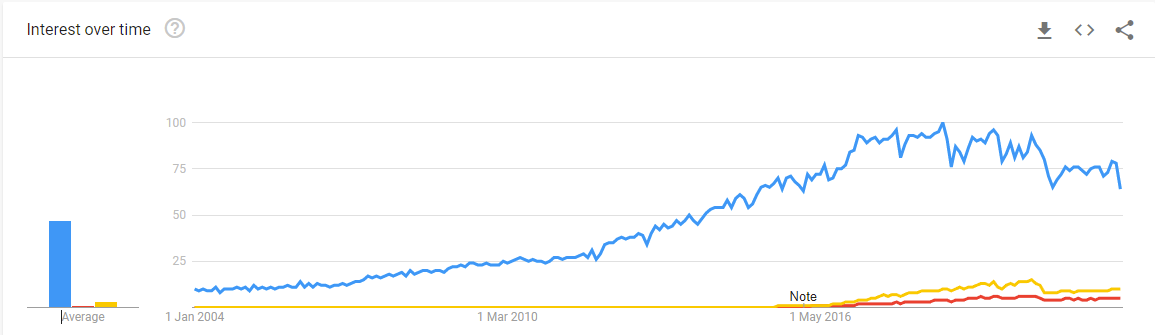
\includegraphics[width=\linewidth]{img/interest_trend.png}
    \caption{Google Trends: REST (modrá), GraphQL (žlutá) a gRPC (červená) \cite{google-trends}}
	\label{google_trends_img}
\end{figure}

\section{REST}
REST je velmi oblíbený architektonický styl pro tvorbu API, který vyniká svou jednoduchostí a čitelností. Na rozdíl např. od gRPC není orientován procedurálně, ale datově.

Zkratka REST vyjadřuje pojem \textit{representational state transfer} a v roce 2000 ji zavedl Roy Fielding ve své dizertační práci \cite{fielding00}. Než vysvětlím, jaké požadavky musí REST API splňovat, je potřeba vysvětlit co to je \textit{zdroj (resource)}.

Jakákoli informace, kterou lze pojmenovat, může být zdrojem. Může to být například obrázek, dočasná služba nebo kolekce jiných zdrojů. Stav zdroje v čase nazýváme reprezentace zdroje. Skládá se ze tří částí -- dat, metadat popisující tato data a hypermedia odkazů, která pomáhají klientům s přechodem do dalšího požadovaného stavu.

REST API by mělo splňovat následující architektonická omezení \cite{restful_api}:

\subsection{Uniform Interface}
Aplikováním principu generality na rozhraní komponenty můžeme zjednodušit architekturu celého systému. Tomu pomáhá několik omezení.
\begin{itemize}
    \item \textbf{Identifikace zdrojů} -- Rozhraní musí jednoznačně identifikovat každý zdroj, který je použit v interakci mezi klientem a serverem.
    \item \textbf{Manipulace se zdroji skrz jejich reprezentaci} -- Zdroje v odpovědi serveru by měly mít jednotnou reprezentaci. Konzumenti API by pak měli použít tyto reprezentace k modifikování stavu zdrojů.
    \item \textbf{Samopopisující se zprávy} -- Každá reprezentace zdroje by měla obsahovat dostatek informací, aby bylo jasné, jak ji zpracovat. Měla by také obsahovat jaké další možné operace může klient se zdrojem provádět.
    \item \textbf{Hypermedia jako aplikační stav} -- Klient by měl mít pouze počáteční URI aplikace. Klientská aplikace by poté měla řídit veškeré interakce pomocí hyperlinků -- serverová odpověď obsahuje seznam dostupných operací.
\end{itemize}

\subsection{Client-server}
Návrhový vzor klient-server vynucuje oddělení zodpovědností, což pomáhá tomu, aby se klientské a serverové komponenty mohly vyvíjet nezávisle na sobě. Zatímco se server a klient vyvíjí, je potřeba dávat pozor, aby rozhraní mezi nimi nebylo porušeno.
Oddělením uživatelského rozhraní (klienta) a manipulaci s daty (serveru) umožníme nezávislost uživatelského rozhraní na konkrétní platformě a zároveň zlepšíme škálovatelnost serveru zjednodušením jeho komponent. Servery nebo klienti mohou být také nahrazeny, pokud nedojde ke změně rozhraní.

\subsection{Stateless}
Bezestavovost požaduje, aby každý požadavek z klienta na server obsahoval všechny dostupné informace potřebné k jeho zpracování. Server nemůže využívat žádných uložených informací z předchozích interakcí -- chová se jako kdyby každý požadavek byl úplně nový. Z toho vyplývá, že klient je zodpovědný za udržování aplikačního stavu, pokud to je potřeba.

\subsection{Cacheable}
Toto omezení požaduje, aby každá odpověď serveru byla označená jako cachovatelná nebo necachovatelná. Pokud je cachovatelná, klient má po omezenou dobu právo tyto informace přepoužít v dalších požadavcích.

\subsection{Layered system}
REST umožnuje využití vrstvené architektury, kde například server A obsahuje API, na serveru B se ukládají data a na serveru C se autentizují požadavky. Klient nemůže zjistit, jestli je ke konkrétnímu serveru připojen přímo nebo přes prostředníka.

\subsection{Code on demand -- volitelné}
Umožnění rozšíření funkcionality klienta stažením a spuštěním kódu ve formě appletů nebo skriptů ze serveru. Výsledkem je zjednodušení klienta, který nemusí obsahovat tolik předinstalovaných funkcí.

\subsection{HTTP}
Pro přenos dat mezi klientem a serverem se nejčastěji používá protokol HTTP, i když REST není vázaný na tento protokol. Protože se ale tato práce zabývá pouze webovými API, budu se v této práci věnovat pouze přenosu pomocí HTTP.
HTTP definuje množinu metod, které slouží k indikaci, jakou akci chceme se zdrojem provést. Tyto metody se také označují jako \textit{HTTP verbs} \cite{http_metods}

\begin{itemize}
    \item \textbf{GET} -- slouží k získání reprezentace daného zdroje. Měla by být použita pouze k získávání informací.
    \item \textbf{HEAD} -- slouží k získání stejné odpovědi jako \textbf{GET}, ale bez těla odpovědi.
    \item \textbf{POST} -- slouží k odeslání entity k danému zdroji, která často způsobí změnu stavu nebo side-effect na serveru.
    \item \textbf{PUT} -- tato metoda nahradí všechny současné reprezentace cílového zdroje za obsah požadavku.
    \item \textbf{DELETE} -- slouží ke smazání cílového zdroje.
    \item \textbf{PATCH} -- slouží k částečné změně cílového zdroje.
\end{itemize}

Metody, které nemění stav serveru označujeme jako bezpečné. Jedná se hlavně o GET a HEAD. V praxi ale běžně není možné tyto metody na straně serveru implementovat tak, aby neměnily vůbec žádný stav -- může například dojít k zalogování volání metody nebo obnovení cache.

Další kategorie jsou idempotentní metody. Idempotence znamená, že pokud klient provede několik shodných požadavků, všechny budou mít stejný výsledek. Jedná se hlavně o GET, HEAD, PUT a DELETE. To ale neznamená, že server musí na každý požadavek odpovědět stejně.


\subsubsection*{Stavové kódy}
HTTP taktéž definuje stavové kódy odpovědí. Tyto kódy se v REST API využívají k informování klienta o výsledku prováděné operace. Tyto kódy se dělí do pěti kategorií, které se od sebe liší prvním číslem. Kódy začínající číslem 100 jsou informační -- komunikují informace na úrovni transportního protokolu \cite{http_codes}. Kódy začínající číslem 200 informují o úspěšném zpracování požadavku. Kódy s číslem 300 značí, že je potřeba dodatečná akce od klienta. Číslo 400 označuje chybový stav na straně klienta. Poslední jsou pak kódy s číslem 500, které označují chybu na straně serveru. Nejčastěji se setkáme s následujícími kódy:
\begin{itemize}
    \item \textbf{200 OK} -- Požadavek proběhl v pořádku. Na rozdíl od kódu 204 by odpověď měla obsahovat i data, a je závislá na použité metodě. Například pro GET by se mělo jednat o reprezentaci zdroje, zatímco pro POST se může jednat o výsledek operace.
    \item \textbf{201 Created} -- Požadavek proběhl v pořádku a jeho výsledkem je vytvoření zdroje. Typicky se jedná o vytvoření zdroje uvnitř kolekce pomocí POST metody.
    \item \textbf{204 No Content} -- Server naplnil požadavek, ale není potřeba vrátit žádnou hodnotu. Například při operaci DELETE, kdy mažeme zdroj z kolekce. Tělo odpovědi nesmí obsahovat žádná data.
    \item \textbf{400 Bad Request} -- Požadavek je pro server nečitelný. Jedná se o obecný chybový kód, který se použije, pokud žádný jiný není vhodný. Může se například jednat o špatný formát požadavku. Klient by stejný požadavek neměl opakovat beze změny.
    \item \textbf{401 Unauthorized} -- Klient není ověřen. Požadavek může být opakován s doplněnými informacemi o ověření.
    \item \textbf{403 Forbidden} -- Klient nemá dostatečná práva. Narozdíl od 401, identita klienta je známa.
    \item \textbf{404 Not Found} -- Server nenašel požadovaný zdroj.
    \item \textbf{405 Method Not Allowed} -- Klient použil metodu, kterou daný zdroj nepodporuje. Odpověď musí obsahovat hlavičku s výčtem podporovaných metod.
    \item \textbf{500 Internal Server Error} -- Server narazil na neočekávanou chybu při zpracování požadavku. Jedná se o obecný chybový kód. Nikdy se nejedná o chybu klienta a dává smysl stejný požadavek opakovat s očekáváním jiné odpovědi.
    \item \textbf{503 Service Unavailable} -- Server není připravený zpracovat požadavek.
\end{itemize}

\section{GraphQL}
GraphQL bylo vytvořeno společností Facebook v roce 2012. Hlavním důvodem jeho vzniku byla narůstající potřeba API pro získávání dat, které bude dostatečně silné a zároveň bude jednoduché na používání. V roce 2015 pak bylo GraphQL zpřístupněno jako open-source \cite{graphql_fb}. Od této doby vznikla spousta implementací v různých jazycích jako je JavaScript, Java, Python a mnoha dalších. GraphQL sestává z typového systému, dotazovacího jazyka, statické validace a typové introspekce.

Data aplikace si můžeme představit jako graf -- jednotlivé entity představují uzly grafu a vztahy mezi nimi pak hrany. Dotazy nad tímto grafem reprezentují strom, který je podgrafem tohoto grafu. Pole, jejichž hodnoty nás zajímají jsou pak listy tohoto stromu. Odtud pochází i samotný název GraphQL -- Graph Query Language.

\subsection{Základní vlastnosti}
\subsubsection*{Definuje strukturu dat}
První věcí, kterou si na GraphQL můžeme všimnout je to, že struktura dat posílaných na server se velmi podobá struktuře dat vrácených v odpovědi, viz obrázek \ref{graphql-query}. To přispívá ke zjednodušení psaní dotazů -- pokud víme jaká data server potřebuje -- a také víme jaký formát dat očekávat. To je jedna z velkých výhod GraphQL, klient si určuje formát dat posílaných ze serveru a má tak přizpůsobená data pro své požadavky.

\begin{figure}[h]
    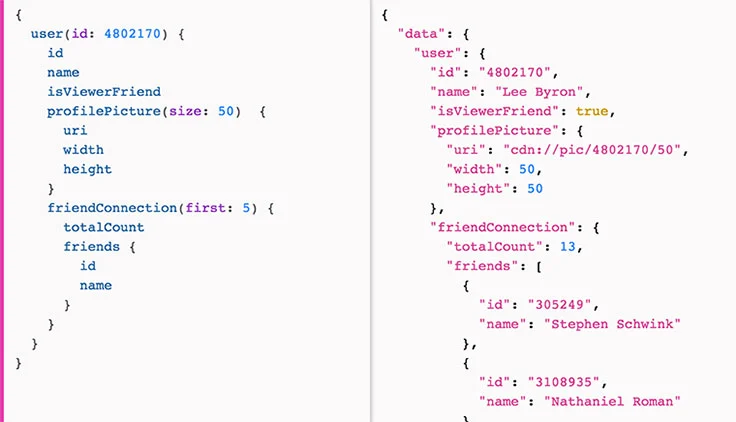
\includegraphics[width=\linewidth]{img/graphql-query.png}
    \caption{Příklad GraphQL dotazu a odpovědi \cite{graphql_query_img}}
	\label{graphql-query}
\end{figure}

\clearpage

\subsubsection*{Hierarchický}
Dalším důležitým aspektem GraphQL je jeho hierarchičnost. Přirozeně totiž sleduje vztahy mezi objekty a oproti RESTu tak dovoluje vyhnout se několikanásobnému volání API pro získání dat souvisejících objektů.

\subsubsection*{Silně typový}
Každý GraphQL server definuje typový systém, který je specifický pro aplikaci.
Každá úroveň GraphQL dotazu odpovídá určitému typu a každý typ má definovanou množinu atributů, které obsahuje. Toto umožňuje validaci dotazů ještě před odesláním na server a zobrazování relevantních chybových hlášek.

\subsection{Protokol, ne úložiště}
Každému atributu v GraphQL na serveru odpovídá nějaká funkce. Pokud už máme existující logiku aplikace společně s úložištěm, můžeme toto všechno na GraphQL napojit.

\subsection{Introspekce}
Díky typovému systému máme možnost prozkoumávat schéma a zjistit dostupné \textit{dotazy (query)}, \textit{mutace (mutation)} nebo \textit{předplatná (subscription)}. Schéma také slouží jako smlouva mezi frontendem a backendem definující jak spolu budou komunikovat.
Introspekce také vytváří platformu pro různé nástroje -- od generování kódu po tvorbu dokumentace.

\subsubsection*{Bez verzí}
Pokud v REST API chceme zachovat stávající funkčnost klientů při přidávání nových funkcionalit, je potřeba zavést verzování API. V praxi je to často řešeno prefixem s číslem verze v URI zdroje,\\*např. \mintinline{text}{http:localhost/v1/products}. S přibývajícím počtem verzí pak roste náročnost úprav API -- pokud budeme například opravovat chybu v aplikaci, je potřeba zajistit, že chyba bude opravena ve všech verzích API, což je velmi časově náročné.

Pokud v GraphQL navrhneme API chytře, tomuto problému se vyhneme. Protože klient si určuje podobu dat sám, server může být jednodušší a obecnější. Místo upravování stávajících funkcionalit, které by poškodily stávající kompatibilitu, budeme přidávat nové. Tento přístup funguje hlavně proto, že podobu vrácených dat si určuje klient, což zabrání případnému nabobtnávání. Atributy, které dále už nebudou podporovány mohou být označeny dekorátorem \mintinline{text}{@deprecated} jako zastaralé a dále budou fungovat, aby nebyla porušena zpětná kompatibilita. Díky těmto postupným změnám máme možnost vyhnout se verzování API.

\subsection{Typový systém}
Protože GraphQL není závislé na konkrétním programovacím jazyku, definuje svoje vlastní typové schéma -- typicky v souboru \mintinline{text}{schema.gql}
Hlavním stavebním prvkem schémat je \textit{Object type}. To je obecný typ, který obsahuje několik dalších atributů. Jeho definice může vypadat následovně. 

\begin{listing}[H]
\begin{minted}{gql.py:GraphqlLexer -x}
type Cart {
  id: Float!
  items: [CartItem!]!
  totalPrice: Float!
  userId: Float!
}
\end{minted}
\caption{GraphQL -- definice typu}
\label{lst:graphql_type}
\end{listing}

\begin{itemize}
    \item \textbf{Cart} definuje \textit{Object type}.
    \item \textbf{id} je typu Float. Vykřičník znamená, že tento atribut je \textit{non-nullable}, což slibuje, že hodnota vždy bude odpovídat danému typu, v tomto případě \textit{Float}.
    \item \textbf{items} reprezentuje pole typu \textit{CartItem}. CartItem je další uživatelem definovaný \textit{Object type}.
    \item \textbf{totalPrice} a \textbf{userId} jsou opět typu \textit{Float}.
\end{itemize}

Každý atribut typu \textit{Object type} může mít libovolný počet argumentů. Každý z těchto argumentů má své jméno. Narozdíl třeba od JavaScriptu, kde funkce přebírají seznam seřazených argumentů, v GraphQL jsou předávány jménem.

I když ve schématu bude nejvíce zastoupen \textit{Object type}, existují ještě tři velmi důležité typy -- \textit{Query}, \textit{Mutation} a \textit{Subscription}. Jedná se o jediné typy operací, které v GraphQL můžeme provádět.

Query se používá pouze pro čtení dat ze serveru, nesmí měnit stav serveru. Mutation se naopak používá právě když je potřeba stav serveru modifikovat. Přirovnáme-li to k RESTu, query jsou obdobou k metodě \mintinline{text}{GET} a mutation k \mintinline{text}{POST}, \mintinline{text}{PUT} nebo \mintinline{text}{DELETE}. Mutation také může vracet data, ale ta by měla být relevantní k prováděné operaci.
Posledním typem je Subscription. Stejně jako dotazy, subscription slouží k získávání dat, ale rozdíl je v tom, že se jedná o dlouho trvající operace. Udržují aktivní spojení se serverem a umožňují tak serveru notifikovat klienta o změnách objektů, ke kterým se přihlásil. Subscription jsou vhodné hlavně pro real-time data -- například sledování ceny akcií.

\begin{listing}[H]
\begin{minted}{gql.py:GraphqlLexer -x}
type Query {    
  getProduct(id: Float!): Product!
}

type Mutation {
  addProduct(newProductData: NewProductInput!): Product!
}
\end{minted}
\caption{GraphQL -- Query a Mutation}
\label{lst:graphql_query_mutation}
\end{listing}

Na příkladě výše je definován dotaz \mintinline{text}{getProduct}, který slouží k získání detailu produktu podle jeho identifikátoru. Níže je pak definována mutace \mintinline{text}{addProduct}, která slouží k vytvoření nového produktu na základě uživatelského vstupu. Tyto typy si jsou syntakticky dost podobné -- největší rozdíl je v názvu operace.

Stavebním prvek typového systému je typ \textit{Scalar}, reprezentující listy dotazů. Mezi skalární typy v GraphQL patří:
\begin{itemize}
    \item Int: celé číslo
    \item Float: desetinné číslo se znaménkem
    \item String: UTF-8 zakódovaný řetězec
    \item Boolean: hodnota true nebo false
\end{itemize}
V mnoha implementacích GraphQL existuje možnost pro definici vlastních skalárních typů. Často je potřeba definovat si typ pro reprezentaci data a času. Je pak naší zodpovědností zajistit serializaci, deserializaci a validaci tohoto typu. Výčtový typ \textit{Enum} je speciálním skalárním typem a slouží reprezentaci dat, která mohou nabývat pouze několika předem daných hodnot. 

Typ \textit{Input} pak ještě slouží k definování dat, která poskytuje uživatel v dotazu a má podobné vlastnosti jako \textit{Object type}.

\subsection{Dotazovací jazyk}
GraphQL je deklarativní jazyk. To znamená, že specifikujeme jak výsledek má vypadat, místo postupu, jak by měl být nalezen. Nejlépe je to vidět na příkladu. Uvažujme následující dotaz:

\begin{listing}[H]
\begin{minted}{gql.py:GraphqlLexer -x}
query {
  allProducts(
      productFilterData: { minPrice: 20, maxPrice: 100 }
    ) {
      name
      price
      status {
        name
      }
    }
}
\end{minted}
\caption{GraphQL -- příklad dotazu}
\label{lst:graphql_query_example}
\end{listing}

Na první řádce specifikujeme, že se jedná o dotaz. Dále je pak potřeba specifikovat jméno dotazu \mintinline{text}{allProducts}, za kterým následuje objekt se vstupními daty pro filtrování produktů -- v tomto případě se jedná o minimální a maximální cenu produktu -- \mintinline{text}{minPrice} a \mintinline{text}{maxPrice}. Poté už jen následuje objekt se samotným výčtem atributů, jejichž hodnoty chceme získat.

Můžeme si všimnout, že atribut \mintinline{text}{status} je typu \mintinline{text}{Object}. Protože všechny typy listů dotazu musí být skalární objekty, je zde potřeba určit nějakou podmnožinu atributů, které skalární budou, jinak by dotaz skončil chybou. Aby se dotaz mohl vyhodnotit, je vždy potřeba specifikovat alespoň jeden atribut.

Na příkladu níže můžeme vidět výsledek tohoto dotazu. Pokud se podařilo dotaz v pořádku provést, najdeme odpověď vždy v objektu \mintinline{text}{data}. Snadno nahlédneme, že odpověď serveru je skutečně velmi podobná struktuře původního dotazu. Hlavními rozdíly jsou absence vstupních dat a to, že produkt je obalený v hranatých závorkách -- to proto, že tento dotaz vrací pole objektů.

\begin{listing}[H]
\begin{minted}{ts}
"data": {
  "allProducts": [
    {
      "name": "Striped Cotton-Blend Socks",
      "price": 25,
      "status": {
        "name": "New"
      }
    }
  ]
}
\end{minted}
\caption{GraphQL -- příklad odpovědi}
\label{lst:graphql_example_response}
\end{listing}

\subsection{Statická validace}
Díky definovanému schématu je jednoduché validovat dotazy -- klient snadno rozpozná, zda nějaký dotaz je validní, a to právě ještě před odesláním na server. Typickými chybami mohou být chybějící vstupní data, přistupování k atributům nějakého skalárního atributu nebo naopak nepřistupování k žádnému atributu neskalárního objektu.

\subsection{Introspekce}
\begin{sloppypar}
Introspekce dovoluje dotazování API pro informace o schématu bez nutnosti čtení dokumentace. Je možné si tak zobrazit dotazy, typy polí nebo direktivy, které server podporuje. Velmi to usnadní práci vývojářům, ale pokud se k našemu API dostane nějaký útočník, dostává zdarma dokumentaci jak server využít. Je tedy vhodné introspekci zakázat v produkčním prostředí.
\end{sloppypar}
Introspekci mohou využívat i různé nástroje -- například díky ní můžeme mít interaktivního klienta pro testování našeho API, který nám bude doporučovat jaké dotazy jsou dostupné  nebo jaké atributy se vyskytují na dané úrovni v dotazu.

\begin{listing}[H]
\begin{minted}{gql.py:GraphqlLexer -x}
{
  __schema {
    types {
      name
      description 
    }
  }
}
\end{minted}
\caption{GraphQL -- ukázka introspekce}
\label{lst:graphql_introspection}
\end{listing}

\section{gRPC}
Google remote procedure call -- gRPC -- je open-source RPC systém původně vyvinutý společnostní Google v roce 2015. RPC v překladu znamená volání vzdálené procedury. Klientská aplikace tedy může volat nějakou proceduru na serveru tak, jako kdyby to byl lokální objekt.

Technologie gRPC je následníkem RPC systému Stubby, který Google používal pro propojení velkého množství mikroslužeb napříč svými datacentry po více než desetiletí \cite{grpc}. Stubby ale nebyl nijak standardizován a byl až příliš úzce závislý na interní infrastruktuře na to, aby ho Google mohl zpřístupnit veřejnosti. S rozvojem technologií jako je \mintinline{text}{HTTP/2} a dalších, bylo rozhodnuto, že je čas Stubby přepracovat.

\begin{figure}[H]
    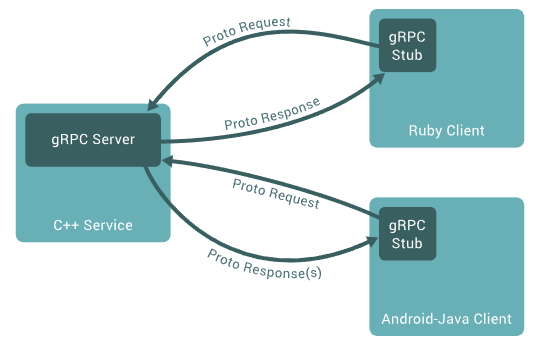
\includegraphics[width=\linewidth]{img/grpc-overview.png}
    \caption{Příklad komunikace serveru a různých klientů \cite{grpc_image}}
	\label{grpc-overview}
\end{figure}

\subsection{Principy a požadavky}
Níže jsem vybral několik hlavních principů a požadavků, na jejichž základě gRPC vzniklo. Všechny jsou pak dostupné na \cite{grpc_requirements}.
\begin{itemize}
    \item \textbf{Služby a zprávy} -- Podpora filozofie mikroslužeb a snaha od oproštění se od problémů s distribuovanými objekty.
    \item \textbf{Pokrytí a jednoduchost} -- gRPC by mělo být dostupné na všech populárních vývojových platformách a zároveň dostatečně jednoduché pro implementaci na vlastní platformě.
    \item \textbf{Zdarma a otevřené} -- všechny základní funkcionality by měly být dostupné zdarma.
    \item \textbf{Interoperabilita a dosah} -- protokol musí být schopný přežít cestu internetem.
    \item \textbf{Obecné a výkonné} -- gRPC musí být vhodné pro velkou škálu způsobů užití a zároveň musí zůstat výkonné.
    \item \textbf{Vrstvené} -- klíčové vrstvy protokolu se musejí vyvíjet nezávisle na sobě. Nesmí se stát, že úprava na síťové vrstvě způsobí přerušení chodu na vrstvě aplikační.
    \item \textbf{Blokující a neblokující operace} -- podpora synchronní a asynchronní komunikace mezi klientem a serverem je klíčová.
    \item \textbf{Standardizované stavové kódy} -- omezení množiny stavových kódů si klade za cíl jasnější ošetřování chyb.
\end{itemize}

\subsection{Protocol buffer}
Protože gRPC je multiplatformní, můžeme mít například server implementovaný v Javě a pak několik klientských aplikací napsaných v různých jazycích, např. JavaScriptu nebo Ruby, viz obrázek \ref{grpc-overview}. Aby mohla klientská aplikace volat vzdálené metody na serveru jako lokální, je potřeba zavést v jakém formátu si budou server a klient vyměňovat zprávy. K tomu se využívají \textit{Protocol buffer}, i když je možné využívat i jiné formáty, pokud je to potřeba. Jedná se o open-source mechanizmus od Googlu říkající jak serializovat strukturovaná data.

Prvním krokem je definice struktury zpráv v \mintinline{text}{.proto} souboru -- jedná se o obyčejný textový soubor s koncovkou \mintinline{text}{.proto}. Základním stavebním prvkem jsou zprávy. To je nejmenší logický celek obsahující dvojice jméno a hodnota nazývané pole. Každá definice pole obsahuje typ, jméno a číslo pole. Soupis všech dostupných skalárních typů je k dispozici zde \cite{proto_scalars}

\begin{listing}[H]
\begin{minted}{protobuf}
message Product {
  int64 id = 1;
  string name = 2;
  string description = 3;
  int64 price = 4;
  int64 quantity = 5;
  repeated ProductCategory categories = 6;
  ProductBrand brand = 7;
  ProductStatus status = 8;
}
\end{minted}
\caption{Příklad protobuf zprávy}
\label{lst:protobuf_example}
\end{listing}

Každé pole má svoje unikátní číslo. Toto číslo identifikuje pole serializované v binárním formátu a nesmí se změnit, jinak by došlo k přerušení fungování existujících klientů. Protože k zakódování čísel polí od 1 do 15 nám stačí jediný bajt (tento bajt ještě obsahuje typ pole), je vhodné tato čísla použít pro pole, která se ve zprávách budou vyskytovat velmi často. Může být dobrý nápad si některá čísla nechat volná pro budoucí potřebu.

Jedna věc, na kterou je potřeba si dát pozor při navrhování zpráv, je že pokud při parsování zprávy nějaký element chybí, jeho odpovídající pole bude naplněno výchozí hodnotou. Pro skalární pole po parsování nemůžeme určit zda se tato výchozí hodnota ve zprávě skutečně vyskytovala nebo nebyla vůbec nastavena. 

Jakmile máme definované zprávy, je potřeba použít kompilátor pro protocol buffer \mintinline{text}{protoc}, který pak vygeneruje přístupové třídy v našem zvoleném jazyce. Tyto třídy pak obsahují metody na získávání a nastavování dat do zpráv a také metody na serializaci a deserializaci.

\subsubsection*{Definice služeb}
gRPC je stejně jako většina RPC systémů založena na myšlence definování služeb, které pak definují své metody a jejich parametry. Služby mohou obsahovat metody čtyř typů:

\begin{itemize}
    \item \textbf{Unary} -- Klient pošle jeden požadavek na server a server mu pošle jednu odpověď zpět.
    \item \textbf{Server streaming} -- Klient pošle jeden požadavek na server a odpovědí získá stream, ve kterém mu server zašle sekvenci zpráv. Klient čte data tak dlouho dokud mu chodí zprávy.
    \item \textbf{Client streaming} -- Klient zasílá sekvenci zpráv na server. Jakmile klient dokončí posílání zpráv, počká až je server přečte a vrátí mu odpověď.
    \item \textbf{Bidirectional streaming} -- Klient a server posílají sekvenci zpráv pomocí read-write streamu. Tyto dva streamy operují nezávisle na sobě, takže klient a server mohou číst a posílat zprávy v jakémkoli pořadí.
\end{itemize}

Jako první věc, kterou musíme udělat, je specifikovat verzi protocol bufferu. Následně můžeme v proto souboru nadefinovat služby a metody, které budou dostupné klientům.

\begin{listing}[H]
\begin{minted}{protobuf}
syntax = "proto3";

service ProductRegister {
  rpc GetProduct (GetProductRequest) 
    returns (GetProductResponse) {};
}
\end{minted}
\caption{Definice gRPC služby}
\label{lst:grpc_service}
\end{listing}

Metoda musí být vždy definována uvnitř nějaké služby -- na příkladě  výše se jedná o službu \mintinline{text}{ProductRegister}. Poté už můžeme definovat samotnou metodu -- první je klíčové slovo \mintinline{text}{rpc}, za kterým následuje jméno metody. A poté nadefinujeme vstupní a výstupní parametry této metody, které musí být typu zpráva.

\subsubsection*{Kompilace protocol bufferu}
Uvažujme zprávu \mintinline{text}{Product} z příkladu \ref{lst:protobuf_example} s polem  \mintinline{text}{name} a cílový jazyk JavaScript. Kompilátor pak vygeneruje třídu \mintinline{text}{Product} s metodou \\* \mintinline{js}{setName(value)} a dalšími potřebnými metodami.

Protoc kompilátor poté ke kódu protocol buffer zpráv také vygeneruje gRPC klientský a serverový kód. Výstup kompilátoru pak záleží na naší zvolené platformě. Pro jazyk C++ vygeneruje odpovídající .h a .cc soubory s třídou pro každou zprávu definovanou v proto souboru. Pro Javu dojde k vygenerování odpovídajících Java tříd společně se speciální Builder třídou sloužící k výrobě instancí tříd jednotlivých zpráv.

Pokud však chceme používat gRPC s jazykem JavaScript, máme na výběr dva způsoby. Prvním je načítat dynamicky deskriptory služeb a klientských stubů přímo ze samotných \mintinline{text}{.proto} souborů pomocí knihovny \\* \mintinline{text}{@grpc/proto-loader}.
Druhý způsob je použití kompilátoru. Dříve zmíněný kompilátor protoc bohužel nepodporuje JavaScript a je potřeba použít kompilátor \mintinline{text}{grpc_tools_node_protoc}, který je dostupný ve správci balíčků npm. Ten pak vygeneruje třídy zpráv a metody na jejich manipulaci.

\subsection{Chybové kódy}
Obdobně jako HTTP, gRPC definuje množinu chybových kódů \cite{grpc_codes}. Následující kódy jsou vhodné pro ošetřování chyb při implementaci API, protože nikdy nejsou vygenerovány gRPC knihovnou.

\begin{itemize}
  \item \textbf{3 INVALID\_ARGUMENT} -- klient poskytl neplatný argument.
  \item \textbf{5 NOT\_FOUND} -- požadovaná entita nebyla nalezena.
  \item \textbf{6 ALREADY\_EXISTS} -- klient se pokusil o vytvoření existující entity.
  \item \textbf{9 FAILED\_PRECONDITION} -- operace byla zamítnuta, protože server není v požadovaném stavu pro její vykonání. V případě API e-shopu se může jednat např. o zamítnutí vytvoření objednávky z prázdného košíku.
  \item \textbf{10 ABORTED} -- operace byla zrušena, typicky kvůli problému souběžnosti -- např. zrušení databázové transakce.
  \item \textbf{11 OUT\_OF\_RANGE} -- operace byla prováděna mimo platný rozsah -- např. čtení za koncem souboru.
  \item \textbf{15 DATA\_LOSS} -- neobnovitelná ztráta dat.
\end{itemize}

\subsection{Verzování}
Filozofie gRPC je taková, že služby by se měly snažit být co nejvíce zpětně kompatibilní. To má několik výhod -- existující klienti budou nadále fungovat, stačí udržovat pouze jednu verzi služby a další. V gRPC jsou změny kategorizovány do tří kategorií.

\begin{itemize}
    \item \textbf{Non-breaking changes} -- Patří sem například přidání nové služby, metody nebo pole do zprávy.
    \item \textbf{Binary breaking changes} -- Tyto změny jsou non-breaking na úrovni protokolu gRPC, ale je potřeba aktualizovat klienty. Jedná se např. o odstranění pole nebo přejmenování zprávy.
    \item \textbf{Protocol breaking changes} -- Patří sem například přejmenování pole, změna čísla pole nebo odstranění služby.
\end{itemize}

Protocol buffer podporuje verzování API specifikací verze do volitelného označení balíčku, např. \mintinline{text}{package products.v1;}. 

\section{Node.js}
JavaScript byl vytvořen společností Netscape jako skriptovací nástroj pro manipulaci s webovými stránkami uvnitř prohlížeče. Tato společnost se také neúspěšně snažila zavést prostředí \textit{Netscape LiveWire} pro běh JavaScriptu na serveru. Server-side JavaScript se tak stal populární až v roce 2009 s uvedením Node.js.

Node.js \cite{node} je open-source a meziplatformní prostředí pro běh JavaScriptu. Je postavené na Google V8 JavaScript engine \cite{v8}, který je také jádrem prohlížeče Google Chrome.

Node.js aplikace běží v jediném procesu a pro příchozí požadavky nevytváří nová vlákna. Když Node.js provádí I/O operaci, například čtení ze sítě nebo databáze, místo blokování vlákna bude Node.js pokračovat až po vrácení výsledku této operace. Toto umožňuje obsluhovat vysoký počet příchozích spojení bez potřeby správy vláken.

Jedna z největších výhod Node.js je, že umožňuje frontendovým vývojářům, kteří píšou klientský kód v JavaScriptu, psát serverový kód bez nutnosti učit se další jazyk. 
Při psaní JavaScriptu pro Node.js nemáme dostupné žádné objekty jako \mintinline{text}{document} nebo \mintinline{text}{window}, které nam poskytuje prohlížeč. Máme ale kontrolu nad prostředím, můžeme si vybrat jakou verzi Node.js budeme používat a není potřeba řešit podporu pro všechny různé verze prohlížeče.

\subsection{npm}
Výchozím správcem balíčků pro Node.js je npm \cite{npm}, plným jménem node package manager. Alternativou je např. yarn\cite{yarn}. Sestává z klienta pro příkazovou řádku a online databáze balíčků, která se označuje jako \textit{npm registry}.

\subsection{TypeScript}
TypeScript je open-source programovací jazyk založený na JavaScriptu, který vyvinula a udržuje společnost Microsoft \cite{typescript_2015}. V podstatě se jedná o nadmnožinu JavaScriptu, která je rozšířená o statické typování. Protože se jedná o nadmnožinu, validní JavaScriptové programy jsou také platnými TypeScriptovými programy. Před spuštěním je pak TypeScript transpilován do čistého JavaScriptu.

Oproti čistému JavaScriptu přináší TypeScript několik výhod:

\begin{itemize}
  \item \textbf{Včasná detekce chyb} -- díky statickému typování je velké množství chyb detekováno již při transpilaci do JavaScriptu. Výzkum odhalil, že TypeScript odhalí 15 \% běžných chyb při kompilaci \cite{typescript_bugs}.
  \item \textbf{Lepší čitelnost} -- díky typům je možné psát kód, který bude více sebepopisující. Lepší čitelnost ocení hlavně vývojáři pracující v týmech.
  \item \textbf{Podpora IDE} -- vývojová prostředí lépe našeptávají a umožňují lepší navigaci napříč kódem projektu. Poskytují vývojáři také zpětnou vazbu -- některé chyby lze odhalit ještě před kompilací. Protože TypeScript je vyvinutý společností Microsoft, je tento jazyk nejvíce podporován vývojovým prostředím Visual Studio Code, které je také vyvíjené Microsoftem. V současnosti je však TypeScript podporován i mnoha dalšími vývojovými prostředími -- např. WebStorm nebo Atom.
\end{itemize}

S těmito výhodami přichází i několik nevýhod. Na naučení se syntaxi TypeScriptu je nutné věnovat nějaký čas. Typové anotace a \textit{syntactic sugar} přinášejí potřebu napsat více kódu, než by bylo v JavaScriptu nutné. I když proces transpilace je automatizovaný, je nutné před samotným vývojem tento proces nakonfigurovat -- toto může být malá výzva, obzvlášť pro vývojáře, který nemá s TypeScriptem žádné zkušenosti.

Kód TypeScriptu je transpilován do JavaScriptu, takže je možné bez problémů vyvíjet klientské i serverové aplikace. Stačí si pouze správně zvolit cílovou verzi JavaScriptu, do které bude kód transpilován.

\chapter{Dostupné technologie}
V této částí představím populární technologie, pomocí kterých je možné jednotlivá API implementovat a vyberu z nich ty, které k implementaci v této práci použiji. 

\section{REST API}
Přestože je možné vytvořit v Node.js server bez použití frameworku, je vhodné nějaký použít, pokud nemám dobrý důvod proti.
 Můžeme tak využít připravených metod ke směrování, ověřování uživatelů a dalších. Mezi případy kdy bychom framework používat nechtěli můžeme třeba zahrnout server se specifickými požadavky na výkon, kde chceme mít co největší část implementace pod kontrolou.

Mezi nejpoužívanější frameworky pro tvorbu REST API v Node.js patří Express.js, Koa.js nebo Nest.js, které dále představím \cite{rest_trends}.
\subsection{Express.js}
Express.js \cite{express} je open-source framework, vydaný pod MIT licencí, pro tvorbu backendu webových aplikací. Byl založen TJ Holowaychukem v roce 2010 a první verze byla vydána na GitHubu 22. května 2010. S počtem 56 tisíc hvězd na GitHubu se jedná o nejpopulárnější framework pro tvorbu REST API v Node.js.

\begin{listing}[h]
\begin{minted}{ts}
const express = require('express')
const app = express()
const port = 3000

app.get('/', (req, res) => {
  res.send('Hello World!')
})

app.listen(port, () => {
  console.log(`Example app listening on port ${port}`)
})
\end{minted}
\caption{Express.js -- Hello World}
\label{lst:express_hello}
\end{listing}

Ukázka kódu \ref{lst:express_hello} ukazuje jednoduchý \textit{Hello world} server, který při zavolání HTTP metody GET vrátí zprávu \mintinline{text}{Hello World!}. 

Nejdříve je nutné importovat a inicializovat samotný Express a definovat port, na kterém bude server poslouchat. Poté definujeme, jaké metody bude server obsluhovat -- pro přidání dalších metod bychom obdobně nastavili \mintinline{javascript}{app.post('/', ...)} pro metodu POST a další HTTP metody. Tyto metody přijímají jako první parametr cestu(route), na které endpoint bude dostupný, a jako druhý parametr objekty request a response, pomocí kterých lze např. číst vstupní data a nastavovat odpověď serveru. V případě že route je lomítko, endpoint je dostupný na kořenové URL.

Na závěr je ještě potřeba zavolat metodu \mintinline{javascript}{app.listen()}, která má jako parametry port, a callback funkci, která se zavolá, jakmile je server připravený obsluhovat požadavky -- zde se jedná o výpis do konzole, že server poslouchá na zadaném portu.

\subsection{Koa.js}
Koa.js \cite{koa} je framework, který byl navržen týmem Expressu, snažící se vyřešit jeho nedostatky a cílí být co nejmenší, nejexpresivnější a robustní. Na rozdíl od Expressu, Koa v základu neobsahuje přibalený žádný middleware. Podle počtu GitHub hvězd -- 32 tisíc -- se jedná o třetí nejpopulárnější framework pro REST API.

Koa aplikace slouží jako rozhraní pro Node.js http server a stará se registraci middlewaru, error handling a konfiguraci objektů pro request a response.
Middleware jsou funkce, které spouštěny ve stylu zásobníku při zpracování requestu -- request zpracuje middleware, zavoláním funkce \mintinline{javascript}{next()} předá kontrolu dalšímu middlewaru a počká na jeho vykonání. Když už není žádný další middleware, pokračuje middleware v dokončení své funkce.

\begin{listing}[H]
\begin{minted}{ts}
const Koa = require('koa');
const app = new Koa();
const port = 3000

app.use(async ctx => {
  ctx.body = 'Hello World';
});

app.listen(port);
\end{minted}
\caption{Koa.js -- Hello World}
\label{lst:koa_hello}
\end{listing}

Můžeme si všimnout, že Hello World aplikace pro Koa.js vypadá jinak než pro Express. V první fázi také importujeme framework a inicializujeme aplikaci. Koa aplikace ale neobsahuje přímo metody na zpracování requestů, umožňuje pouze definovat middleware pomocí metody \mintinline{javascript}{app.use()}. Middleware v této ukázce kódu pak zpracovává všechny příchozí requesty a nastavuje tělo odpovědi na \mintinline{text}{Hello World}. Objekty Request a Response jsou pak dostupné jako atributy objektu Context pod názvy \mintinline{javascript}{request} a \mintinline{javascript}{response}.

Pokud bychom chtěli zpracovávat requesty přímo pro konkrétní URI a metodu, je potřeba importovat router middleware:

\begin{listing}[H]
\begin{minted}{ts}
import Router     from 'koa-router';
const router = new Router();
router.get('/', async (ctx, next) => {
    await ctx.render('hello-world', context);
});
app.use(router.routes());
\end{minted}
\caption{Koa.js -- Router}
\label{lst:koa_router}
\end{listing}

Stejně jako u Expressu pak specifikujeme HTTP metodu zavoláním obdobné metody na objektu routeru. Poté je potřeba pomocí metody \mintinline{javascript}{app.use()} předat tento middleware samotné aplikaci.

\subsection{Nest.js}
Nest.js \cite{nest} je framework pro tvorbu výkonných, škálovatelných server-side aplikací. Plně podporuje TypeScript a kombinuje prvky objektově orientovaného programování společně s prvky funkcionálního a funkcionálně-reaktivního programování. V základu Nest.js na pozadí využívá Express, ale je možné nakonfigurovat i pro framework Fastify. Se 46 tisíci GitHub hvězdami se jedná o druhý nejpopulárnější REST framework.

Na rozdíl od  výše uvedených frameworků Express.js a Koa.js, které slouží čistě k tvorbě HTTP serverů, Nest.js poskytuje i out-of-the-box aplikační architekturu, která poskytuje velké množství výhod jako: škálovatelnost, snadná udržovatelnost nebo modulárnost. Přináší to ale i jisté nevýhody. V případě že tvoříme mikroslužby, architektura Nest.js může být příliš svazující. To doprovází i strmější učící křivka jako psaní velkého množství boiler-plate kódu, což je možné vidět i na ukázkovém Hello World serveru níže. 

Inicializace Nest.js serveru může vypadat následovně a je na první pohled vidět, že se významně liší od předchozích frameworků.

\begin{listing}[H]
\begin{minted}{ts}
import { NestFactory } from '@nestjs/core';
import { AppModule } from './app.module';

async function bootstrap() {
  const app = await NestFactory.create(AppModule);
  await app.listen(3000);
}
bootstrap();
\end{minted}
\caption{Nest.js -- Bootstrap}
\label{lst:nest_bootstrap}
\end{listing}

Nejdříve je potřeba naimportovat továrnu NestFactory, pomocí které sestavíme naší aplikaci. Dále importujeme Appmodule, který obsahuje logiku aplikace. Nakonec definujeme funkci boostrap, pomocí které server spustíme.

Samotný kód pro obsloužení metody GET bychom pak definovali v controlleru AppController:

\begin{listing}[H]
\begin{minted}{ts}
import { Get, Controller } from '@nestjs/common';

@Controller()
export class AppController {
    @Get()
    hello() {
        return 'Hello World';
    }
}
\end{minted}
\caption{Nest.js -- Hello World}
\label{lst:nest_hello}
\end{listing}

Z výše uvedených frameworků jsem se rozhodl pro implementaci REST API vybrat Express.js. Oproti Nest.js slouží k čistě ke tvorbě API a nenutí vývojáře  dodržovat doporučenou strukturu architektury, což umožní co nejpřímočařejší srovnání s implementacemi pro GraphQL a gRPC. Koa.js by pro tento úkol byl také vhodný, ale zatím hlavní výhoda Expressu je jeho popularita a podpora komunity vývojářů.

\section{GraphQL API}
Stejně jako pro REST, i pro GraphQL existuje množství frameworků pro tvorbu serverů, i když ne tak velké. Mezi nejpoužívanější patří Apollo Server (12 tisíc hvězd), GraphQL Yoga (7 tisíc hvězd) nebo GraphQL Express (6 tisíc hvězd na GitHubu), který je referenční implementací GraphQL serveru \cite{graphql_libraries}.

\subsection{GraphQL Express}
Přestože GraphQL Express \cite{express-graphql} je referenční implementací GraphQL serveru, je až na třetím místě z pohledu oblíbenosti. Oproti ostatním frameworkům na tvorbu GraphQL API neobsahuje tolik funkcionalit a možností nastavení, může být však dobrá volba pro doplnění REST API o GraphQL.

\begin{listing}[H]
\begin{minted}{ts}
var express = require('express');
var { graphqlHTTP } = require('express-graphql');
var { buildSchema } = require('graphql');

var schema = buildSchema(`
  type Query {
    hello: String
  }
`);

var root = { hello: () => 'Hello world!' };

var app = express();
app.use('/graphql', graphqlHTTP({
  schema: schema,
  rootValue: root,
  graphiql: true,
}));
app.listen(4000, 
  () => console.log('Server listening at localhost:4000/graphql')
);
\end{minted}
\caption{GraphQL Express -- Hello World}
\label{lst:graphqljs_hello}
\end{listing}

Na ukázce kódu \ref{lst:graphqljs_hello} můžeme vidět příklad implementace jednoduchého GraphQL serveru. Na začátku je potřeba importovat potřebné balíčky. Dalším krokem je definice GraphQL schématu -- v tomto případě jediného dotazu, který se jmenuje \mintinline{text}{hello}, vrací typ řetězec a neobsahuje žádné vstupní parametry. Poté je potřeba implementovat resolver, který bude tento dotaz vyhodnocovat. Pak už zbývá jen samotná inicializace serveru -- vytvoříme instanci Express serveru a předáme mu middleware, který bude obsluhovat požadavky přicházející na adresu \mintinline{text}{/graphql}. Poslední krok je samotné spuštění serveru.

\subsection{Apollo Server}
Tato implementace GraphQL serveru patří jak mezi nejoblíbenější podle počtu GitHub hvězd, tak i mezi nejstahovanější balíčky z npm. Apollo Server \cite{apollo} je napsaný v TypeScriptu a oproti Express GraphQL obsahuje více funkcionalit. Můžu zmínit například plugin Apollo Playground pro jednoduché a rychlé testování GraphQL API v prohlížeči.

\begin{listing}[H]
\begin{minted}{ts}
const { ApolloServer, gql } = require('apollo-server');
const typeDefs = gql`
    type Query {
        hello: String
    }
`;
const resolvers = {
    Query: {
        hello: () => {
            return 'Hello World!';
        }
    }
};
const server = new ApolloServer({typeDefs, resolvers})
server.listen(4000).then(({ url }) => {
    console.log(`🚀 Server ready at ${url}`);
});
\end{minted}
\caption{Apollo Server -- Hello World}
\label{lst:apollo_hello}
\end{listing}

Jak lze vidět na ukázce kódu \ref{lst:apollo_hello}, inicializace Apollo serveru se od GraphQL Express serveru příliš neliší. Hlavní rozdíl je v definici schématu a resolverů.

\clearpage
\subsection{GraphQL Yoga}
GraphQL Yoga \cite{graphql_yoga} je dalším frameworkem pro tvorbu GraphQL serveru, který se zaměřuje na rychlou konfiguraci, výkon a developer experience. Tento framework byl původně vyvíjen společností Prisma, ale v roce 2021 ho převzala společnost The Guild. Velká výhoda tohoto frameworku je nativní podpora Subscriptions.
\begin{listing}[H]
\begin{minted}{ts}
const { createServer } = require('@graphql-yoga/node')

const server = createServer({
  schema: {
    typeDefs: `
      type Query {
        ping: String
      }
    `,
    resolvers: {
      Query: {
        hello: () => 'Hello World!',
      },
    },
  },
})

server.start()
\end{minted}
\caption{GraphQL Yoga -- Hello World}
\label{lst:yoga_hello}
\end{listing}

Definice GraphQL serveru pomocí frameworku GraphQL Yoga je velmi podobná té z Apollo serveru.

Pro implementaci GraphQL API jsem se rozhodl vybrat serverový framework Apollo GraphQL. Mezi hlavní důvody patří jeho velká oblíbenost a množství dostupné dokumentace.
\clearpage

\section{gRPC API}
Nejmladší z technologií pro tvorbu API probíraných v této práci je gRPC. Toto je velmi znát v omezeném výběru serverů dostupných pro jeho implementaci. Na výběr máme referenční implementací gRPC serveru (3 386 hvězd), minimalistický server pro implementaci mikroslužeb Mali (794 hvězd) nebo server ProtoCat (42 hvězd). Podíváme-li se na počet stažení přes NPM nebo počet hvězd na GitHubu, jejich počty jsou řádově nižší než např. u Expressu.

Pro všechny následující ukázkové implementace gRPC serveru použiji stejnou protobuf definici služby. Jedná se o jednu metodu, která bude vracet odpověď s jedním atributem.

\begin{listing}[h]
\begin{minted}{protobuf}
service Greeter {
  rpc SayHello (HelloRequest) returns (HelloResponse) {}
}
message HelloRequest {}
message HelloResponse {
  string message = 1;
}
\end{minted}
\caption{protobuf -- Hello World}
\label{lst:protobuf_hello}
\end{listing}

\subsection{Referenční implementace gRPC-js}
Referenční implementace gRPC \cite{grpc_js} má zatím největší výhodu v tom, že je nejpoužívanější a je k ní dostupné největší množství dokumentace.
Na ukázce kódu lze \ref{lst:grpcjs_hello} je vidět implementace gRPC služby Greeter s metodou sayHello. Na první pohled je vidět, že oproti RESTu a GraphQL je potřeba napsat nejvíce kódu -- protobuf definici a inicializaci serveru.

Na začátku je potřeba importovat všechny potřebné knihovny. Dalším nutným krokem je konfigurace a samotné načtení definice služeb z \mintinline{text}{.proto} souboru. Poté následuje implementace \mintinline{text}{hello}, která bude později namapována na na metodu \mintinline{text}{sayHello} ze služby \mintinline{text}{Greeter}. Zbývá už jen nakonfigurovat samotný server. Server přidáme službu Greeter s implementací její metody, nastavíme port na kterém bude server naslouchat a můžeme ho spustit.

Samotné načítání \mintinline{text}{.proto} souborů a inicializace serveru pak můžeme zjednodušit použitím frameworků, můžeme však přijít o úroveň granularity konfigurace.

\begin{listing}[h]
\begin{minted}{ts}
var PROTO_PATH = __dirname + '/helloworld.proto';

var grpc = require('@grpc/grpc-js');
var protoLoader = require('@grpc/proto-loader');
var packageDefinition = protoLoader.loadSync(
  PROTO_PATH,
  {
    keepCase: true,
    longs: String,
    enums: String,
    defaults: true,
    oneofs: true
  });
var protoDescriptor = grpc.loadPackageDefinition(
  packageDefinition);
var helloworld = protoDescriptor.helloworld;

function hello(call, callback) {
  callback(null, {
    message: 'Hello World!'
  });
}

function main() {
  var server = new grpc.Server();
  server.addService(helloworld.Greeter.service,
    { sayHello: hello });
  server.bindAsync('0.0.0.0:50051', 
  grpc.ServerCredentials.createInsecure(), () => {
    server.start();
  });
}
\end{minted}
\caption{grpc-js -- Hello World}
\label{lst:grpcjs_hello}
\end{listing}


\subsection{Mali.js}
Mali \cite{mali} je velmi minimalistický framework pro tvorbu gRPC mikroslužeb. Je inspirovaný již zmíněným frameworkem Koa s využitím gRPC konceptů. Jak uvidíme na ukázce kódu \ref{lst:mali_hello}, Mali umožňuje vyhnutí se spoustě boilerplate kódu, který byl potřeba napsat při implementaci pouze s grpc-js.

\begin{listing}[h]
\begin{minted}{ts}
const Mali = require('mali')

function sayHello (ctx) {
  ctx.res = { message: `Hello World!` }
}

function main () {
  const app = new Mali('helloworld.proto')
  app.use({ sayHello })
  app.start('0.0.0.0:50051')
}
\end{minted}
\caption{Mali -- Hello World}
\label{lst:mali_hello}
\end{listing}

Z ukázky kódu \ref{lst:mali_hello} je patrné, že implementace jednoduchého serveru je záležitost na pár řádek kódu. Načítání \mintinline{text}{.proto} souborů si framework řeší sám a stačí mu pouze přidat cestu k nim při inicializaci serveru.

Po importování samotného frameworku implementujeme metodu \\* \mintinline{text}{sayHello}, inicializujeme samotný server, předáme implementaci metody a server spustíme.

\subsection{ProtoCat}
ProtoCat \cite{protocat} je open-source minimalistickým frameworkem pro gRPC.

Oproti předchozím gRPC implementacím nenačítá protobuf definice přímo ze souborů, ale je potřeba vygenerovat příslušné definice, typy pro TypeScript a metody pomocí \mintinline{text}{grpc_tools_node_protoc} kompilátoru.

\begin{listing}[h]
\begin{minted}{ts}
import { ProtoCat } from 'protocat';
import { GreeterService } from '../dist/greeter_grpc_pb';

const app = new ProtoCat()
app.addService(GreeterService, {
  sayHello: async call => {
    call.response.setMessage('Hello World!')
  };
});
  
app.start('0.0.0.0:3000')
\end{minted}
\caption{ProtoCat -- Hello World}
\label{lst:protocat_hello}
\end{listing}

Jako první krok je potřeba importovat samotný framework ProtoCat a poté definici služby, která byla vygenerována protoc kompilátorem. Poté vytvoříme novou instanci serveru a zaregistrujeme novou službu. Můžeme si všimnout, že metoda \mintinline{text}{.setMessage()} byla vygenerována protoc kompilátorem. Pak už stačí pouze samotný server spustit.

Z dostupných frameworků pro gRPC jsem se rozhodl použít ProtoCat, protože definování gRPC služeb mi přišla velmi intuitivní a podporuje TypeScript. %zduvodnit lepe

\chapter{Návrh}
Aby srovnání bylo co nejsnáze představitelné a zároveň reflektovalo běžný způsob užití, rozhodl jsem se pro implementaci API e-shopu. Je to typický příklad, se kterým se vývojář může setkat při své práci a zároveň je tento příklad dost obecný na to, aby si ho čtenář mohl jednoduše převést na jiný. 

Začal jsem s návrhem REST API, pro jehož popis jsem zvolil specifikaci OpenAPI. GraphQL a gRPC API pak budou z tohoto návrhu vycházet -- REST zdrojům budou odpovídat GraphQL Resolvery a gRPC služby.

\section{OpenAPI Specification}
OpenAPI Specification definuje standard pro HTTP aplikační rozhraní, který je nezávislý na konkrétním programovacím jazyce a je čitelný jak pro počítač tak pro člověka.

Díky strojově čitelnému formátu existuje nespočetné množství nástrojů, které programátorům usnadňují práci s API. Tyto nástroje sahají od jednoduchých validátorů, přes mockování serverů, čehož často využívají frontend vývojáři, po generátory zdrojového kódu nebo dokumentace API. To nás přivádí ke dvěma hlavním přístupům navrhování REST API -- \textit{Design First} nebo \textit{Code First} \cite{api_design_approach}.

\begin{itemize}
  \item \textbf{Design first přístup} -- je vhodný zejména tehdy, když záleží na rozšiřitelnosti a znovupoužitelnosti výsledného API. Specifikace zde slouží jako smlouva popisující chování výsledného API. Tento přístup vyžaduje strávení více času nad tím, jak tato smlouva má vypadat. Věnování více času plánování má pak za následek identifikaci klíčových funkcionalit a vyhnutí se nepotřebným funkcionalitám. Jakmile je specifikace připravena ve strojově čitelném formátu, je možné využít nástroje na generování kódu k vygenerování útržků kódů nebo typů, které se pak použijí při vývoji.
  \item \textbf{Code first přístup} -- tento přístup je zejména vhodný, když je kladen velký důraz na rychlost dodání produktu. Plánování specifikace je zde zredukováno na minimum a vývojáři mohou co nejdříve začít pracovat na tvorbě API. Specifikace API je pak generována nějakým nástrojem ze zdrojového kódu. Další výhodou tohoto přístupu je, že specifikace je vždy konzistentní s aktuální verzí API. Oproti design first přístupu ale vývojáři mohou pálit čas na nepotřebných funkcionalitách.
\end{itemize}

V této práci jsem zvolil design first přístup, zejména z důvodu návrhu funkcionalit, na kterých půjdou ukázat rozdíly použitých technologií k tvorbě API.

\section{Návrh API e-shopu}

Začal jsem definováním kroků typického průchodu e-shopem, které je nutné podniknout k úspěšnému odeslání objednávky.

\begin{enumerate}
  \item Zobrazení a filtrování produktů.
  \item Registrace a správa uživatele.
  \item Vložení produktu do košíku.
  \item Vytvoření objednávky.
  \item Správa objednávek.
\end{enumerate}

Následně jsem identifikoval klíčové zdroje a metody, které bude potřeba naprogramovat. Další část popisuje, jaké operace podporuje navržené API. Celá specifikace ve formátu OpenAPI je dostupná v příloze zdrojových kódů této práce.

\subsection{/users}
Tento zdroj slouží k manipulaci s daty uživatelů nebo k registraci nových a přihlašování stávajících uživatelů. Obsahuje následující operace:

\begin{itemize}
  \item \textbf{GET} \mintinline{text}{/users}  -- zobrazení dat uživatelů
  \item \textbf{POST} \mintinline{text}{/users}  -- vytvoření nového uživatele
  \item \textbf{GET} \mintinline{text}{/users/:id} -- zobrazení detailu uživatele určeného identifikátorem
  \item \textbf{PUT} \mintinline{text}{/users/:id} -- úprava dat uživatele určeného identifikátorem
  \item \textbf{DELETE} \mintinline{text}{/users/:id}  -- smazání uživatele určeného identifikátorem
  \item \textbf{POST} \mintinline{text}{/users/login} -- přihlášení uživatele pomocí jména a hesla
  \item \textbf{POST} \mintinline{text}{/users/refresh} -- obnovení přihlašovacího tokenu po vypršení
\end{itemize}

Pro všechny metody kromě vytvoření a přihlášení uživatele je vyžadováno aby byl uživatel přihlášen.

\subsection{/products}
Tento zdroj slouží k listování a manipulaci s daty produktů. Také je možné sledovat skladové množství produktu v reálném čase.

\begin{itemize}
  \item \textbf{GET} \mintinline{text}{/products} -- vylistování dostupných produktů. Podporuje filtrování podle ceny nebo identifikátorů
  \item \textbf{POST} \mintinline{text}{/products} -- vytvoření nového produktu
  \item \textbf{GET} \mintinline{text}{/products/:id} -- zobrazení detailu produktu určeného identifikátorem
  \item \textbf{PUT} \mintinline{text}{/products/:id} -- úprava dat produktu určeného identifikátorem
  \item \textbf{DELETE} \mintinline{text}{/products/:id} -- smazání produktu určeného identifikátorem
  \item \textbf{WebSocket} \mintinline{text}{/products/:id/quantity} -- přihlášení se k real-time odběru informací o skladovém množství produktu
\end{itemize}

Pro zobrazování dat o produktech není vyžadováno přihlašování, pro metody, které mění data, už ano.

\subsection{/categories}
Tento zdroj slouží k zobrazení, tvorbě a úpravě produktových kategorií.

\begin{itemize}
  \item \textbf{GET} \mintinline{text}{/categories} -- zobrazí seznam všech kategorií
  \item \textbf{POST} \mintinline{text}{/categories} -- vytvoření nové kategorie
  \item \textbf{GET} \mintinline{text}{/categories/:id} -- zobrazení detailu kategorie určené identifikátorem
  \item \textbf{PUT} \mintinline{text}{/categories/:id} -- úprava dat kategorie určené identifikátorem
  \item \textbf{DELETE} \mintinline{text}{/categories/:id} -- smazání kategorie určené identifikátorem
\end{itemize}

Obdobně jako u produktů je čtení dat povoleno pro nepřihlášené uživatele, ale pro editaci dat přihlášení potřeba je.

\subsection{/carts}
Tento zdroj slouží ke správě košíku přihlášeného uživatele, podporuje přidávání a úpravu věcí v košíku a vytvoření nové objednávky.

\begin{itemize}
  \item \textbf{GET} \mintinline{text}{/carts/detail} -- zobrazí košík přihlášeného uživatele
  \item \textbf{POST} \mintinline{text}{/carts/addItem} -- přidá zvolený produkt do košíku
  \item \textbf{PUT} \mintinline{text}{/carts/updateItem} -- slouží k úpravě položek přidaných do košíku
  \item \textbf{DELETE} \mintinline{text}{/carts/clearCart} -- vyprázdní obsah košíku
  \item \textbf{POST} \mintinline{text}{/carts/checkout} -- vytvoření nové objednávky
\end{itemize}

Všechny metody tohoto zdroje vyžadují, aby byl uživatel ověřen a dovolují pouze upravování jeho vlastního košíku.

\subsection{/orders}
Tento zdroj slouží ke správě objednávek přihlášeného uživatele.

\begin{itemize}
  \item \textbf{GET} \mintinline{text}{/orders} -- zobrazí seznam všech objednávek přihlášeného uživatele
  \item \textbf{GET} \mintinline{text}{/orders/:id} -- zobrazení detailu objednávky určené identifikátorem
  \item \textbf{PUT} \mintinline{text}{/orders/:id/updateStatus} -- změna stavu existující objednávky
  \item \textbf{DELETE} \mintinline{text}{/orders/:id} -- zrušení objednávky určené identifikátorem
\end{itemize}

Operace s tímto zdrojem může provádět pouze ověřený uživatel.

\subsection{Databázové schéma}
Podle hotového návrhu API jsem pokračoval návrhem databázového modelu. Model databáze jsem navrhoval v ORM nástroji Prisma, který používá speciální jazyk k definování modelu do souboru \mintinline{text}{schema.prisma}.

Na obrázku \ref{schema-dbdiagram} je znázorněna vizualizace databázového schématu pomocí nástroje \mintinline{text}{dbdiagram.io}.

\begin{figure}[h]
  \centerline{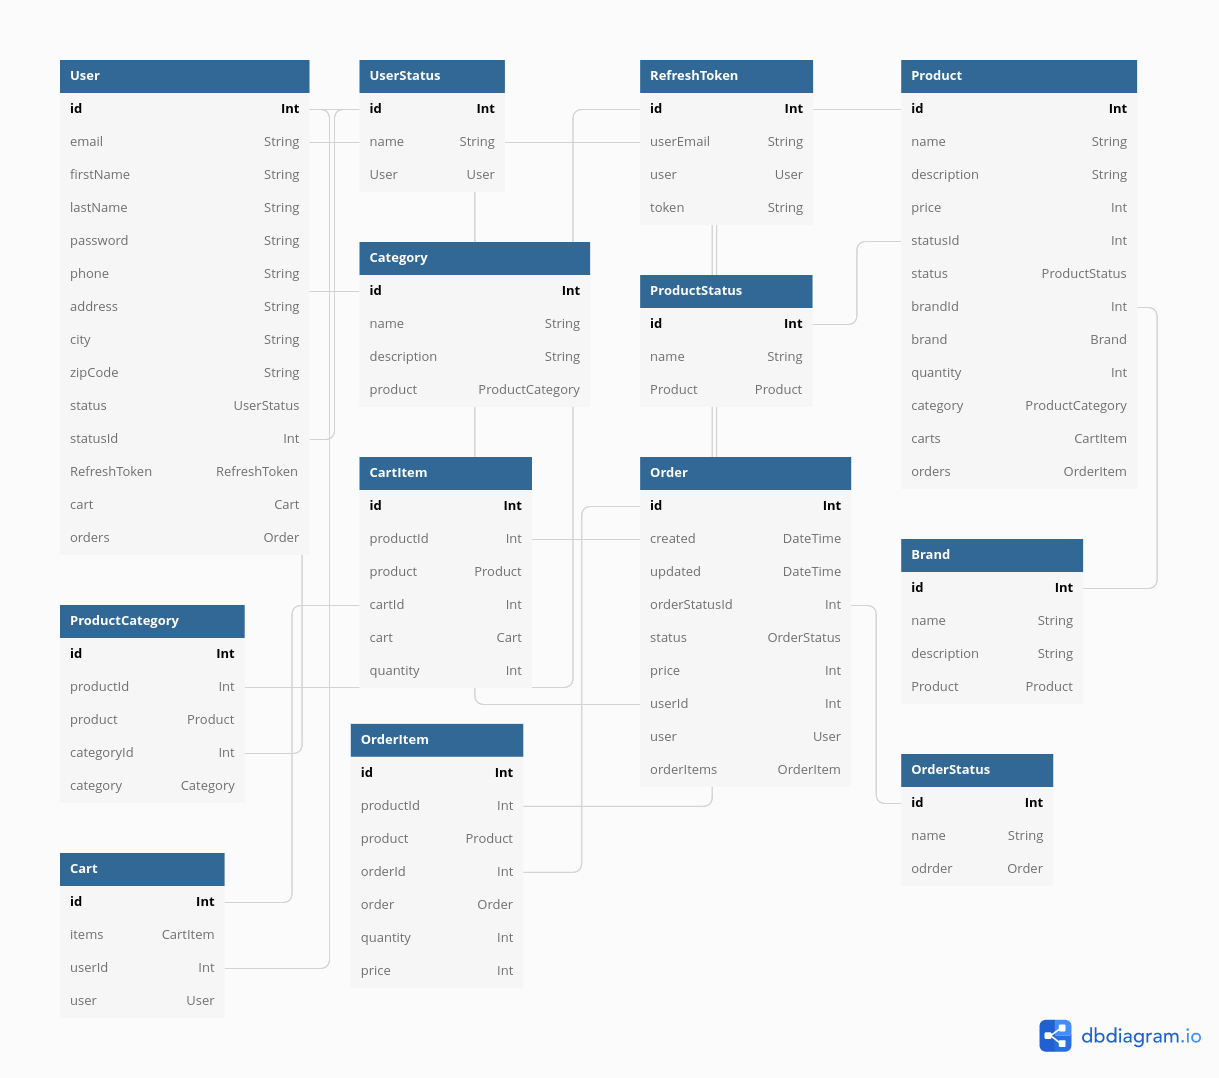
\includegraphics[scale=0.45, angle=90]{img/schema-dbdiagram.png}}
  \caption{Vizualizace DB schématu pomocí nástroje dbdiagram.io}
	\label{schema-dbdiagram}
\end{figure}

\chapter{Implementace}
Tato kapitola popisuje aspekty samotné implementace navrženého API v REST, GraphQL a gRPC.

\section{Datové úložiště}
Pro vyhnutí se potřebě spravování vlastního databázového serveru jsem se rozhodl spouštět databázi, stejně jako jednotlivé implementace API, v Docker kontejneru. To umožňuje jednoduše vytvořit oddělené instance databáze pro jednotlivé implementace API. Další výhodou je jednoduchost instalace, kdy k rozběhnutí databáze na novém počítači stačí stáhnout daný Docker image a spustit ho. Jako databázový systém jsem zvolil PostgreSQL.

\subsection{Prisma}
Pro návrh databázového schématu jsem využil funkce zvolené ORM knihovny Prisma. Ta používá vlastní jazyk na popis modelu, ze kterého se poté vygeneruje SQL a naplní databáze. Prisma podle tohoto modelu vygeneruje odpovídající typy pro TypeScript.

Prvním krokem je samotná inicializace Prismy v projektu. K tomu slouží příkaz \mintinline{text}{npx prisma init}, který udělá následující:
\begin{itemize}
  \item vytvoří složku \mintinline{text}{prisma} -- tato složka obsahuje soubor \mintinline{text}{schema.prisma}, ve kterém bude definováno databázové schéma
  \item vytvoří soubor \mintinline{text}{.env} -- v tomto souboru jsou definovány proměnné prostředí, například spojení do databáze
\end{itemize}

V souboru \mintinline{text}{schema.prisma} je poté nutné specifikovat proměnnou prostředí obsahující přihlašovací údaje do databáze a typ databáze, viz ukázka kódu \ref{lst:prisma_datasource}.

\begin{listing}[H]
\begin{minted}{ts}
datasource db {
  provider = "postgresql"
  url      = env("DATABASE_URL")
}
\end{minted}
\caption{schema.prisma -- datasource}
\label{lst:prisma_datasource}
\end{listing}

Datový model může vzniknout dvěma způsoby -- pokud připojujeme Prismu k existující databázi, je možné vygenerovat model pomocí introspekce \cite{prisma_introspection}. Druhý způsob je navrhnout model ručně. V této práci se budu zabývat pouze ručním návrhem modelu.

Ukázka kódu \ref{lst:prisma_model} pak zobrazuje, jak může definice schématu v Prismě vypadat. Z každého objektu, který je označen klíčovým slovem \mintinline{text}{model}, vznikne v databázi jedna tabulka. Uvnitř modelu jsou poté definované jednotlivé atributy -- ty odpovídají sloupcům v databázi. Znak \mintinline{text}{?} za názvem atributu značí, že se jedná o nepovinný atribut. Tyto atributy jsou pak doplněny o typy (skalární typy nebo reference na jiný Prisma model) a dekorátory. Dekorátory specifikují zvláštní chování -- např. že atribut je identifikátorem a je automaticky inkrementován -- \mintinline{text}{@id @default(autoincrement())}.

\begin{listing}[H]
\begin{minted}{text}
model User {
  id           Int            @id @default(autoincrement())
  email        String         @unique
  firstName    String
  lastName     String
  password     String
  phone        String?
  address      String?
  city         String?
  zipCode      String?
  status       UserStatus     @relation(fields: [statusId],
                                        references: [id])
  statusId     Int
  RefreshToken RefreshToken[]
  cart         Cart?
  orders       Order[]
}
\end{minted}
\caption{schema.prisma -- Příklad modelu}
\label{lst:prisma_model}
\end{listing}

Jakmile je datový model navržen, můžeme příkazem \mintinline{text}{npx prisma migrate} vygenerovat SQL soubor s databázovou migrací, která bude následně aplikována do databáze.

Pak už jen stačí do projektu nainstalovat klienta pro Prismu pomocí příkazu \mintinline{text}{npm install @prisma/client} a všechno je připraveno k dotazování databáze, viz ukázka kódu \ref{lst:prisma_example}. Dotazovat databází lze buď pomocí rozhraní Prisma klienta nebo čistým SQL pomocí metody \mintinline{text}{prisma.$executeRaw}. Spouštění SQL je velmi důležitá funkce a umožňuje řešení problémů, které v klientovi zatím nejsou implementovány. Např. zamykání tabulek během transakcí klient neobsahuje, a proto bylo nutná implementace pomocí SQL zámků.

Prisma klient podporuje zpracování transakcí třemi způsoby. První způsob je pole volání prisma klientů, která budou následně zavolána v jedné transakci. Druhým způsobem jsou interaktivní transakce, kdy klientu předáme celou funkci, která proběhne v rámci jedné transakce. Třetím je pak ruční správa transakcí pomocí čistého SQL. 

Interaktivní transakce jsem použil při implementaci vytvoření objednávky, kdy je potřeba během transakce kontrolovat počet položek skladem, aby nešla vytvořit objednávka s více položkami než je možné. Bohužel tato vlastnost je zatím ve fázi vývoje a při výkonnostním testu se mi podařilo objevit chybu, která způsobovala deadlock a timeout transakce. Tato chyba by však měla být v další verzi Prismy opravena.

\begin{listing}[H]
\begin{minted}{ts}
export const prisma = new PrismaClient();
const cart = await prisma.cart.findUnique({
  where: {
    userId: 1,
  },
});
\end{minted}
\caption{Prisma -- inicializace klienta a dotaz}
\label{lst:prisma_example}
\end{listing}

\section{REST API -- Express.js}
Express umožňuje obsluhovat požadavky aplikace na úrovni celé aplikace ve formátu \mintinline{text}{app.get('/user'...)}, ale to se stává velmi nepřehledné s narůstající komplexitou aplikace. Proto jsem se rozhodl implementaci strukturovat na Express Routery, které obsluhují dané zdroje. Ke každému zdroji přísluší definice typů a služba, ve které je implementována samotná logika metod. Ke každému routeru pak přísluší sada testů kontrolující jeho implementaci.

Ukázka kódu \ref{lst:express_init} ukazuje inicializaci express serveru, použití middlewaru \mintinline{text}{morgan} k logování příchozích požadavků, middlewaru \mintinline{text}{json} k parsování těl příchozích požadavků, a nakonec přimountování všech routerů.

\begin{listing}[H]
\begin{minted}{ts}
export const app = expressWs(express()).app;

app.use(morgan("tiny"));
app.use(express.json());

app.use("/users", usersRouter);
app.use("/products", productsRouter);
app.use("/categories", categoriesRouter);
app.use("/carts", cartsRouter);
app.use("/orders", ordersRouter);

\end{minted}
\caption{Express -- inicializace aplikace}
\label{lst:express_init}
\end{listing}

Každý Router pak může obsluhovat požadavky pouze na zadané cestě. Na ukázce kódu \ref{lst:express_router} je vidět definice a implementace routeru pro zdroj \mintinline{text}{/carts}, konkrétně metody POST pro přidávání položek do košíku.

Middleware pro routery jde definovat buď na úrovni celého routeru, stejně jako to je na ukázce, nebo jdou jednotlivé middlewary předávat na úrovni metody a cesty, pokud je potřeba větší granularita.

Příkazem \mintinline{text}{app.use("/carts", cartsRouter);}, kde \mintinline{text}{app} je instance Express serveru, je pak možné router přimountovat k serveru.

\begin{listing}[H]
\begin{minted}{ts}
export const cartsRouter = express.Router();

cartsRouter.use(verifyToken);

cartsRouter.post("/addItem",
    async (req: Request, res: Response) => {
  try {
    const cartItem = new NewCartItemInput(req.body);
    await validate(cartItem).then((errors) => {
      if (errors.length > 0) {
        throw new BadRequestError(`Invalid input: ${errors}`);
      }
    });
    const newItem = await CartService.addItem(
      req.user.user_id, cartItem);
    return res.status(201).json(newItem);
  } catch (e) {
    handleError(e, res);
  }
});
\end{minted}
\caption{Express -- router}
\label{lst:express_router}
\end{listing}

Ke kontrole vstupních dat používám knihovnu \mintinline{text}{class-validator}, která umožňuje doplnit JavaScriptové třídy o dekorátory, které popisují, jak by měl formát dat vypadat. Poté lze pak zavoláním metody \mintinline{js}{validate(input)} zkontrolovat, zda uživatelský vstup obsahuje všechna data. Umožňuje také kontrolu hodnot, například jestli se jedná o email.

Poté co vstupní data projdou kontrolou, jsou předána do služby, v případě v ukázce se jedná o \mintinline{text}{CartService}, ve které je implementována logika práce s košíkem uživatele. Tato služba pak vrátí výsledek, který Router posílá v odpovědi. Výhodou oddělení implementace logiky od samotného routeru je nezávislost na implementaci

\subsection{Error Handling}
Na kód na úrovni jednotlivých metod v routerů jsem obalil do try catch bloku, ve kterém odchytávám všechny výjimky, které během volání mohou nastat. Odchycené výjimky jsou pak obslouženy v metodě \mintinline{text}{handleError}, která nastavuje odpovídající tělo odpovědi a mapuje tyto výjimky na správné HTTP status kódy.

\subsection{Ověřování uživatelů}
Implementoval jsem vlastní systém pro ověřování uživatelů s využitím knihovny \mintinline{text}{jsonwebtoken}. Uživatel se přihlásí požadavkem na endpoint \mintinline{text}{/users/login}, kde se zkontroluje shoda hashí uloženého a poskytnutého hesla pomocí knihovny \mintinline{text}{bcrypt}. Pokud je přihlášení úspěšné, uživateli je vygenerován JWT token, pomocí kterého pak může přistupovat na další endpointy. V tokenu jsou pak zakódovány informace o uživateli, čehož lze využít při kontrole, zda má uživatel oprávnění číst daný zdroj. Tento token je pak potřeba nastavit do hlavičky požadavku na \mintinline{text}{x-access-token}. Dále je uživateli vygenerován RefreshToken pro obnovení ověřovacího tokenu po jeho vypršení bez nutnosti zadávat znovu přihlašovací údaje.

K samotnému ověření uživatele jsem implementoval middleware, který nejdříve kontroluje, zda požadavek obsahuje ověřovací token. Pokud požadavek token obsahuje, následuje dekódování tokenu a rozšíření objektu požadavku o informace o přihlášeném uživateli. V opačném případě požadavek skončí chybou ověření.


\subsection{WebSocket}
Express nativně nepodporuje WebSockety. Pro implementaci WebSocketů jsem zvolil knihovnu \mintinline{text}{express-ws}, která umožňuje použití routerů i pro WebSockety. Při inicializaci Express serveru ho pak stačí předat jako parametr této knihovně.

WebSocket router je pak definován obdobně jako klasický router, s výjimkou toho, že místo HTTP metod se použije metoda \mintinline{text}{.ws()}, viz ukázka kódu \ref{lst:ws_router}.

Pro demonstraci WebSocketů jsem implementoval endpoint \\* \mintinline{text}{products/:id/quantity}, který umožňuje klientům zaregistrovat se k real-time odběru informací o skladové dostupnosti produktu. Využil jsem k tomu \mintinline{text}{EventEmitter} z knihovny \mintinline{text}{events}, který umožňuje posílat notifikace a zaregistrovat se k jejich odběru. Pokaždé, když je změněn počet dostupných položek daného produktu, je vyslána notifikace. Lze poslouchat buď všechny notifikace, nebo se přihlásit k odběru jen určitých uživatelem definovaných typů -- v tomto případě se jedná o typ \mintinline{text}{update}.

\begin{listing}[h]
\begin{minted}{ts}
productsRouter.ws("/:id/quantity", async (ws, req: Request) => {
  try {
    const id: number = parseInt(req.params.id, 10);
    const quantity = await ProductService.getQuantity(id);
    const data = {
      timestamp: Date.now(),
      quantity: quantity,
    };
    ws.send(JSON.stringify(data));
    productEmmiter.on("update", async () => {
      const updatedProduct = await ProductService.find(id);
      const data = {
        timestamp: Date.now(),
        quantity: updatedProduct.quantity,
      };
      ws.send(JSON.stringify(data));
    });
  } catch (e) {
    logger.error(e);
    let message = "Server error";
    if (e instanceof Error) {
      message = e.message;
    }
    ws.send(`${message}. Terminating connection`);
    ws.terminate();
  }
});
\end{minted}
\caption{WebSocket router}
\label{lst:ws_router}
\end{listing}

\subsection{Testy}
Pro testování API jsem zvolil knihovnu \mintinline{text}{jest} spolu s knihovnou \mintinline{text}{supertest}, která slouží jako klient pro testování webových API. Supertestu je předán jako parametr samotný server a pak jsou nad ním volány odpovídající metody. Na následující ukázce \ref{lst:test_rest} se posílá GET požadavek, pomocí metody \mintinline{text}{set()} je do hlavičky nastaven ověřovací token. Poté následuje kontrola výsledku. Metodou \mintinline{text}{expect(200)} se ověří hodnota HTTP stavového kódu. Poté následuje pomocí metod \mintinline{text}{expect()} kontrola dat v těle odpovědi.

\begin{listing}[H]
\begin{minted}{ts}
await supertest(app)
  .get("/carts/detail")
  .set("x-access-token", token)
  .expect(200)
  .then(async (res) => {
    expect(res.body.userId).toBe(1);
    expect(res.body.items.length).toBe(2);
    expect(res.body.totalPrice).toBe(4855);
  });
\end{minted}
\caption{Testování REST API}
\label{lst:test_rest}
\end{listing}


\section{GraphQL API -- Apollo Server}
Při tvorbě GraphQL API máme na výběr dva přístupy -- design first a code first -- a podle nich výběr dostupných knihoven. Protože REST API jsem měl už navržené a implementované, rozhodl jsem se vydat přístupem code first. K tomu jsem využil knihovnu \mintinline{text}{type-graphql}. Tato knihovna umožňuje automatické vygenerování GraphQL schématu, stačí k tomu pouze doplnit psaný kód o dekorátory. Kromě generování schématu, dekorátory dělají kód čitelnější a jednodušší. Pokud k danému dotazu má mít přístup jen ověřený uživatel, stačí použít dekorátor \mintinline{text}{@Authorized()}.

Rozhodl jsem se pro podobnou strukturu aplikace jako při implementace REST API, s tím rozdílem, že GraphQL nepoužívá routery, ale resolvery.

\subsection{Inicializace serveru}
Před samotným spuštěním serveru je potřeba vytvořit GraphQL schéma. Protože využívám code first přístupu, schéma se sestavuje automaticky pomocí metody \mintinline{text}{buildSchema} z knihovny \mintinline{text}{type-graphql}. Ta přijímá za parametry implementované resolvery, implementaci ověřování uživatelů, formát serializace data, příznak, jestli se vygenerované schéma má uložit do souboru a jako poslední příznak, zda se má implicitně spouštět validace pomocí dekorátorů z knihovny \mintinline{text}{class-validator}.

K inicializaci serveru je potřeba předat vygenerované schéma, pluginy (pokud jsou potřeba, v tomto případě používám plugin Apollo Playground pro zjednodušení testování API) a context, ve kterém je možné definovat vlastní middleware. Poté je server připravený na spuštění příkazem \mintinline{text}{server.start()}

\begin{listing}
\begin{minted}{ts}
const schema = await buildSchema({
  resolvers: [CartResolver, CategoryResolver,
    OrderResolver, ProductResolver, UserResolver],
  authChecker: authChecker,
  dateScalarMode: "isoDate",
  emitSchemaFile: true,
  validate: false,
});

const server = new ApolloServer({
  schema,
  plugins: [ApolloServerPluginLandingPageGraphQLPlayground],
  context: ({ req }) => {
    const context = {
      req,
      user: req.user,
    };
    return context;
  },
});
\end{minted}
\caption{GraphQL -- inicializace serveru}
\label{lst:example}
\end{listing}

\begin{listing}[H]
\begin{minted}{ts}
@Resolver(Product)
export class ProductResolver {
  @Authorized()
  @Mutation((returns) => Product)
  async updateProduct(
    @Arg("id") id: number,
    @Arg("updateProductData") updateProductData: UpdateProductInput,
    @PubSub() pubSub: PubSubEngine
  ) {
    const updatedProduct = await ProductService.update(
      id, updateProductData);
    await pubSub.publish("PRODUCT", updatedProduct);
    return updatedProduct;
  }
}
\end{minted}
\caption{GraphQL -- Resolver}
\label{lst:graphql_resolver}
\end{listing}

Na ukázce \ref{lst:graphql_resolver} je vidět příklad resolver pro manipulaci s produkty. Třída resolveru je obalena dekorátorem, který popisuje že se jedná o resolver a jaký typ obsluhuje. Uvnitř resolveru následuje implementace mutace pro editaci dat produktů. Ta je doplněna dekorátorem, který označuje že se jedná o mutaci společně s jejím návratovým typem. Následuje samotná implementace mutace, kde vstupní parametry jsou označeny dekorátory \mintinline{text}{@Arg()} a PubSubEngin, který je použit k implementaci subscription, která je popsána dále. Pak už zbývá samotná implementace logiky, která je delegována službě ProductService a vrácení výsledku.

O kontrolu vstupních hodnot se stará sama knihovna \mintinline{text}{type-graphql}, díky definici typů a dekorátorům. Samozřejmě, že kdybychom potřebovali nějakou sofistikovanější kontrolu, musíme si ji sami implementovat, např. pomocí dříve zmíněného \mintinline{text}{class-validatoru}. 

\begin{listing}[H]
\begin{minted}{ts}
@InputType()
export class UpdateProductInput {
  @Field({ nullable: true })
  name: string;
  @Field({ nullable: true })
  description: string;
  @Field({ nullable: true })
  price: number;
  @Field({ nullable: true })
  quantity: number;
  @Field((type) => [Int], { nullable: true })
  categoryIds: number[];
  @Field({ nullable: true })
  brandId: number;
  @Field({ nullable: true })
  statusId: number;
}
\end{minted}
\caption{GraphQL -- InputType}
\label{lst:graphql_inputtype}
\end{listing}

Dekorátor \mintinline{text}{@InputType()} u třídy označuje, že se jedná o typ, ve kterém budou přicházet uživatelem zadaná data. Každé pole, je pak potřeba doplnit o dekorátor \mintinline{text}{@Field()}, který obsahuje informaci, zda je pole povinné a jeho typ (pokud nejde zjistit pomocí reflexe).

\subsection{Error Handling}
Ošetřování chyb je součást GraphQL specifikace a je součástí výchozí implementace GraphQL odpovědí. K označování chybových stavů používám výjimky definované v knihovně \mintinline{text}{apollo-server-core}, které jsou doplněny o vhodnou chybovou hlášku a jsou pak zpracovány Apollo Serverem.

\subsection{Ověření uživatele}
Stejně jako v REST implementaci používám i zde k ověřování uživatelů knihovnu \mintinline{text}{jsonwebtoken}. Uživatelé se přihlašují zasláním požadavku na mutaci \mintinline{text}{loginUser}, která jim vrátí přístupový token a token k jeho obnovení. Ověřovací middleware se pak stará o rozšíření objektu požadavků o data přihlášeného uživatele. Knihovna \mintinline{text}{type-graphql} obsahuje funkci na kontrolu ověření uživatelů, kde je možné si doimplementovat další funkce jako např. kontrola přístupových práv. Tato kontrola se pak aktivuje dekorátorem \mintinline{text}{@Authorized()}, který jde umístit na úroveň resolveru, dotazu nebo mutace.

\subsection{GraphQL subscription}
Apollo Server nepodporuje nativně subscriptions, proto je potřeba vytvořit vlastní WebScocket server, který bude subscriptions obsluhovat. Samotné definování subscription je pak vcelku jednoduché, viz ukázka \ref{lst:graphql_subscription}. V dekorátoru \mintinline{text}{@Subscription} určíme jaké téma toto subscription obsluhuje a volitelnou filtrovací funkci -- v tomto případě filtruje produkty, k jejichž notifikaci o změně jsme se přihlásili. Poté už následuje samotná implementace vrácení výsledku. Můžeme si všimnout, že oproti implementaci v REST API, implementace subscription vyžaduje výrazně méně kódu.

V předchozí ukázce \ref{lst:graphql_resolver} je demonstrováno poslání notifikace subscription enginu. Knihovna Prisma ve své první verzi obsahovala implementaci subscriptions. Tato funkce ale už v nových verzích není dostupná.

\begin{listing}[H]
\begin{minted}{ts}
@Authorized()
@Subscription({
  topics: "PRODUCT",
  filter: ({ payload, args }) => {
    return args.productIds.includes(payload.id);
  },
})
quantityUpdate(
  @Root() product: Product,
  @Args() args: QuantityUpdateArgs): Product {
    return product;
}
\end{minted}
\caption{GraphQL -- Subscription}
\label{lst:graphql_subscription}
\end{listing}

\subsection{Testy}
K implementaci testů pro GraphQL jsem také použil kombinaci knihoven \mintinline{text}{jest} a \mintinline{text}{supertest}. Samotné testování probíhá obdobně, kdy supertest slouží jako klient, který volá jednotlivé dotazy a mutace. Největší rozdíl je v samotném odesílání požadavků -- nejdříve je nutné sepsat celý dotaz, který musí obsahovat všechna pole, které chceme zobrazit, a poté jsou všechny dotazy posílány na jediný endpoint na serveru. Díky konstrukci dotazovacího řetězce vyžaduje psaní testů pro GraphQL napsat větší množství kódu a času.

\section{gRPC API -- ProtoCat}
Implementace gRPC je ukázkovým příkladem design driven přístupu, protože nejdříve je potřeba definovat strukturu API v protobuf souborech a až poté je možné pracovat na implementaci. Implementace pro REST byla rozdělena na jednotlivé routery, GraphQL na resolvery a u gRPC je rozdělená na jednotlivé služby. Každé této službě odpovídá jeden \mintinline{text}{.proto} soubor.

Jakmile jsou tyto služby nadefinovány, je potřeba z nich vygenerovat kód, který použijeme při implementaci serveru. Pro kompilaci těchto souborů je vhodné nastavit např. npm script abychom se vyhnuli opakovanému psaní dlouhého příkazu s mnoha argumenty viz \ref{lst:protobuf_comp}. Příkaz nejdříve smaže a znovu vytvoří složku pro vygenerované soubory, poté následuje samotná kompilace -- pomocí parametrů můžeme nastavit styl vygenerovaného JavaScriptu, TypeScriptu.

\begin{listing}[h]
\begin{minted}{text}
rm -rf ./dist/api &&
mkdir -p ./dist/api &&
grpc_tools_node_protoc 
  --js_out=import_style=commonjs,binary:./dist/api
  --ts_out=generate_package_definition:./dist/api
  --grpc_out=grpc_js:./dist/api
  -I ./src/proto ./src/proto/**/*.proto"
\end{minted}
\caption{Protobuf kompilace}
\label{lst:protobuf_comp}
\end{listing}


Kompilátor vytvoří pro každý \mintinline{text}{.proto} soubor jednu složku, která obsahuje čtyři soubory -- JavaScript implementaci zpráv a gRPC služeb a odpovídající TypeScript definice, které jsou potřeba jako pro implementaci služeb na serveru, tak i pro klienta.


\subsection{Inicializace serveru}
Inicializace ProtoCat serveru je pak záležitost na několik řádek kódu, viz ukázka \ref{lst:grpc_init}. Nejdříve je potřeba vytvořit instanci serveru. 
Poté můžeme pokračovat přidáním middlewaru, v tomto případě používám middleware pro ověřování uživatelů. Pak následuje registrace implementovaných gRPC služeb, pro které jsem si vytvořil vlastní metody (samotná implementace služby je v ukázce kódu \ref{lst:grpc_service}). Nakonec pak stačí spustit server příkazem \\* \mintinline{text}{app.start("0.0.0.0:3000")}, kterému jako parametr zadáme adresu a port.

\begin{listing}
\begin{minted}{ts}
export const app = new ProtoCat<ServerContext>();

app.use(authMdw);

addCartServiceRegister(app);
addCategoryServiceRegister(app);
addOrderServiceRegister(app);
addProductServiceRegister(app);
addUserServiceRegister(app);
\end{minted}
\caption{gRPC -- inicializace serveru}
\label{lst:grpc_init}
\end{listing}


Ukázka kódu \ref{lst:grpc_service} zobrazuje definici metody \mintinline{text}{updateProduct} ve službě \mintinline{text}{ProductRegisterService}. Metoda nejdříve zkontroluje, jestli je uživatel přihlášený a poté načte vstupní data. Třída \mintinline{text}{UpdateProductInput} je wrapper třída pro vstupní data, která využívá vygenerovaných metod pro načtení vstupních dat z gRPC zprávy. Poté jsou vstupní data zkontrolována pomocí knihovny \mintinline{text}{class-validator} a předána do ProductService, která implementuje logiku API, stejně jako tomu bylo v předchozích případech. Zbývá už jen notifikovat emitter o aktualizaci produktu a vrátit výsledek. Pro nastavení výsledku zde používám další wrapper metodu, která nastavuje příslušné atributy do gRPC zprávy s odpovědí.

Pro každý atribut ve zprávě totiž protoc kompilátor vygeneroval metody na jeho získání a nastavení. Pro každý z těchto atributu je pak tedy potřeba zavolat jeho odpovídající metodu s hodnotou, na kterou ho chceme nastavit.

\begin{listing}
\begin{minted}{ts}
app.addService(ProductRegisterService, {
  updateProduct: async (call) => {
    if (!call.user || !call.user.id) {
      throw new UnauthorizedError("Unauthorized");
    }
    const updateProductInput = 
        new UpdateProductInput(call.request);
    await validate(updateProductInput).then((errors) => {
      if (errors.length > 0) {
        throw new InvalidArgumentError("Invalid input");
      }
    });
    const product = await ProductService.update(
      updateProductInput.id, updateProductInput);
    productEmmiter.emit("update", product.quantity);
    call.response.setProduct(createProductResponse(product));
  }
})
\end{minted}
\caption{gRPC -- Definice služby}
\label{lst:grpc_service}
\end{listing}

\subsection{Error Handling}
Pro zachytávání a obsluhu výjimek jsem si implementoval vlastní middleware, který zachytává mou definované výjimky. Middleware pak definované výjimky mapuje na odpovídající gRPC stavové kódy a nastavuje odpovídající metadata.

\subsection{Ověření uživatele}
Pro přihlašování uživatelů slouží metoda \mintinline{text}{loginUser} ve službě \\* \mintinline{text}{UserRegisterService}. Obdobně jako u předchozích implementací, tato metoda vrací ověřovací JWT token společně s tokenem na jeho obnovu po vypršení. K ověřování uživatelů jsem si pak implementoval vlastní gRPC middleware, který po úspěšném ověření uživatele doplní objekt zprávy o jeho data.

Ověřovací token se nastavuje v metadatech do atributu \mintinline{text}{authorization}. Metadata jsou gRPC obdobou HTTP hlavičkám.

\subsection{gRPC streaming}
ProtoCat implementuje streaming nativně díky podpoře \mintinline{text}{HTTP/2} a není k tomu potřeba nastavovat žádný další server. Pro porovnání s předchozími implementaci jsem si vybral server streaming (odpovídá GraphQL subscription).

Pro implementaci streamingu je nejdříve nutné popsat metodu pro streaming v protobuf souboru, viz ukázka \ref{lst:grpc_stream}. To že se jedná o stream poznáme podle toho, že definice gRPC metody obsahuje klíčové slovo stream buď v požadavku (client streaming), v odpovědi (server streaming) nebo v obou (bidirectional streaming).

\begin{listing}
\begin{minted}{protobuf}
rpc GetProductQuantityStream (GetProductQuantityStreamRequest)
  returns (stream GetProductQuantityStreamResponse) {};
\end{minted}
\caption{gRPC -- stream}
\label{lst:grpc_stream}
\end{listing}

Pak už můžeme implementovat samotnou metodu pro streamování,\\* viz ukázka \ref{lst:grpc_stream implementation}. Prvním krokem je z požadavku získat identifikátor produktu, u kterého budeme sledovat jeho dostupné množství. Pro odpověď vytvoříme novou instanci vygenerované třídy \mintinline{text}{GetProductQuantityStreamResponse} a nastavíme hodnotu dostupných produktů. Data pak pošleme klientovi zavoláním metody \mintinline{text}{write}. Potom obdobně jako u implementace WebSocketu i zde využívám \mintinline{text}{EventEmitter} z knihovny \mintinline{text}{events}. Ten naslouchá notifikace typu update, a jakmile vyhodnotí dostupné množství produktu, pošle ho zpět klientovi.

\begin{listing}[H]
\begin{minted}{ts}
getProductQuantityStream: async (stream) => {
  const id = stream.request.getId();
  const product = await ProductService.find(id);
  const response = new GetProductQuantityStreamResponse()
    .setQuantity(product.quantity);
  stream.write(response);
  productEmmiter.on("update", async (quantity) => {
    if (!quantity) {
      const updatedProduct = await ProductService.find(1);
      quantity = updatedProduct.quantity;
    }
    response.setQuantity(quantity);
    stream.write(response);
  });
}
\end{minted}
\caption{gRPC -- stream implementation}
\label{lst:grpc_stream implementation}
\end{listing}

\subsection{Testy}
Pro testování gRPC API využívám knihovnu \mintinline{text}{jest}. Bohužel zde nelze využít knihovny \mintinline{text}{supertest} pro testování HTTP API a bylo potřeba implementovat vlastního gRPC klienta pro účely testování. Poté bylo ještě potřeba pomocí beforeAll a afterAll metod spustit a zastavit gRPC server.

ProtoCat umožnuje velmi snadnou inicializaci klienta, viz \ref{lst:grpc_client}. Opět zde využívá vygenerované implementace pomocí protoc kompilátoru. Metodě \\* \mintinline{text}{createClient} předáme implementace klienta pro služby, které chceme používat, adresu s portem, na které server běží a přístupové údaje k serveru.

\begin{listing}[H]
\begin{minted}{ts}
const client = createClient(
  {
    category: CategoryRegisterClient,
    user: UserRegisterClient,
  },
  ADDRESS,
  ChannelCredentials.createInsecure()
);
\end{minted}
\caption{gRPC -- klient}
\label{lst:grpc_client}
\end{listing}

\clearpage
Ukázka \ref{lst:gRPC_client_call} ukazuje jak lze klienta použít. Přes objekt služby přistoupíme k metodě, kterou chceme zavolat a předáme jí jako parametr metodu, která nastavuje metada a atributy požadavku, které jsme si vygenerovali pomocí protoc kompilátoru.

\begin{listing}[H]
\begin{minted}{ts}
const { response } = await 
    client.category.getCategory((req, metadata) => {
  metadata.set("authorization", token);
  req.setId(2);
});
\end{minted}
\caption{gRPC -- použití klienta}
\label{lst:gRPC_client_call}
\end{listing}

\chapter{Výkonnostní testování}
Pro výkonnostní testování jsem využil nástroj k6 od Grafana Labs \cite{k6}. K6 jako jeden z mála dostupných nástrojů pro zátěžové testování umožňuje testování REST, GraphLQ a gRPC API bez nutnosti instalace dodatečných pluginů. K programování testů se používá JavaScript a není tak potřeba učit se další syntaxi a umožňuje použití populárních JavaScript knihoven.

Testování pomocí tohoto nástroje probíhá tak, že pomocí JavaScriptu si definujeme scénář testu, který pak poskytneme K6 jako parametr společně s konfigurací samotného testu -- např. délce testu, počet procesů, které se spustí.

Bohužel tento nástroj zatím nepodporuje testování gRPC streamů, a tak bylo nutné pro test streamování implementovat vlastní testovací skript.

Každý ze tří serverů byl spuštěn v Docker kontejneru s vlastní Postgres databází, která byla taktéž spuštěna v Docker kontejneru.

Počítač, na kterém testování probíhalo měl následující parametry:

\begin{itemize}
  \item operační systém Ubuntu 20.04.4 LTS 64bit
  \item procesor Intel® Core™ i5-8350U CPU @ 1.70GHz $\times$  8 
  \item operační paměť 16GB
  \item grafická karta Mesa Intel® UHD Graphics 620 (KBL GT2)
\end{itemize}

Každý test jsem třikrát zopakoval a výsledek zprůměroval, abych se vyhnul případným anomáliím při měření.

\clearpage
\section{Zobrazení detailu produktu}
Test probíhal s 10 virtuálním uživateli běžícími paralelně po dobu 30 s. Každý virtuální uživatel po vyhodnocení požadavku pokračoval odeslání dalšího. Z výsledků na obrázku \ref{test_get_product} můžeme vidět, že nejrychleji požadavky odbavovaly REST a GraphQL API, přibližně stejnou rychlostí. gRPC bylo nejpomalejší, přisuzuji to režii při serializaci a deserializaci zpráv.

\begin{figure}[]
  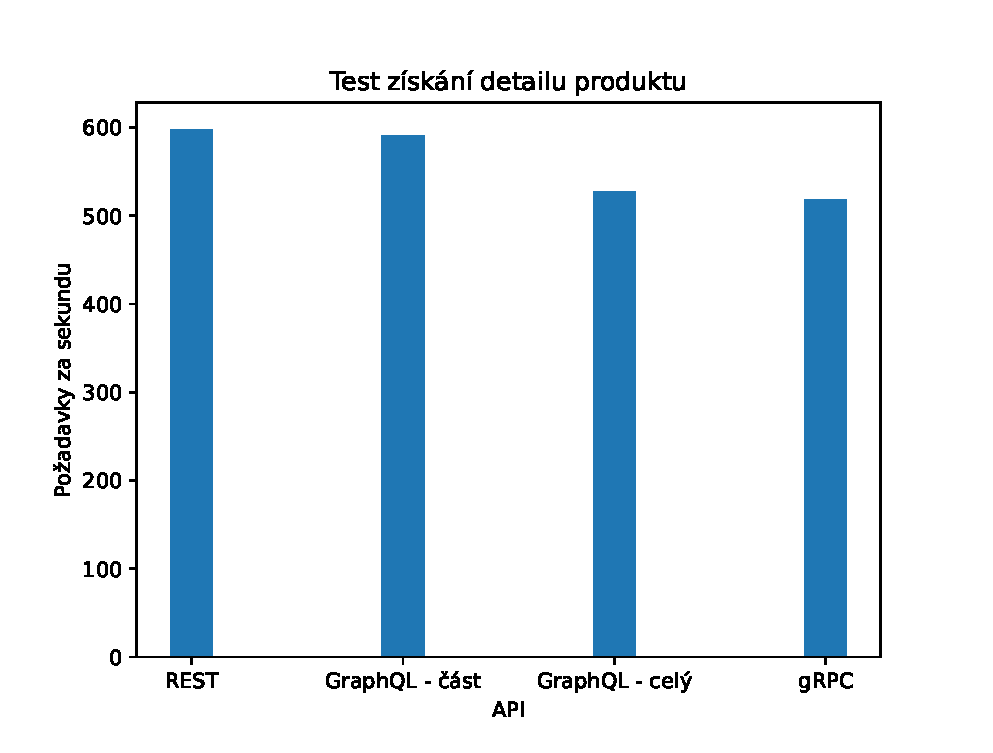
\includegraphics[width=\linewidth]{img/get-product.eps}
  \caption{Detail produktu -- Počet odbavených požadavků za sekundu}
\label{test_get_product}
\end{figure}

Na grafu \ref{test_get_product} lze vidět porovnání velikostí požadavků a odpovědí pro zobrazování detailu produktu.

Požadavky nejmenší velikosti mělo gRPC a následně REST. GraphQL požadavky měly největší velikost, zejména kvůli nutnosti specifikace tvaru dotazu. 

Nejmenší velikost odpovědi mělo opět gRPC API, což přisuzuji kompresi dat při serializaci odpovědí. Následovalo GraphQL s omezenou podmnožinou polí v odpovědi. Na třetím místě se pak umístil REST. Největší velikost odpovědi pak měly GraphQL dotazy, které obsahovaly všechny pole produktu.

\begin{figure}[]
  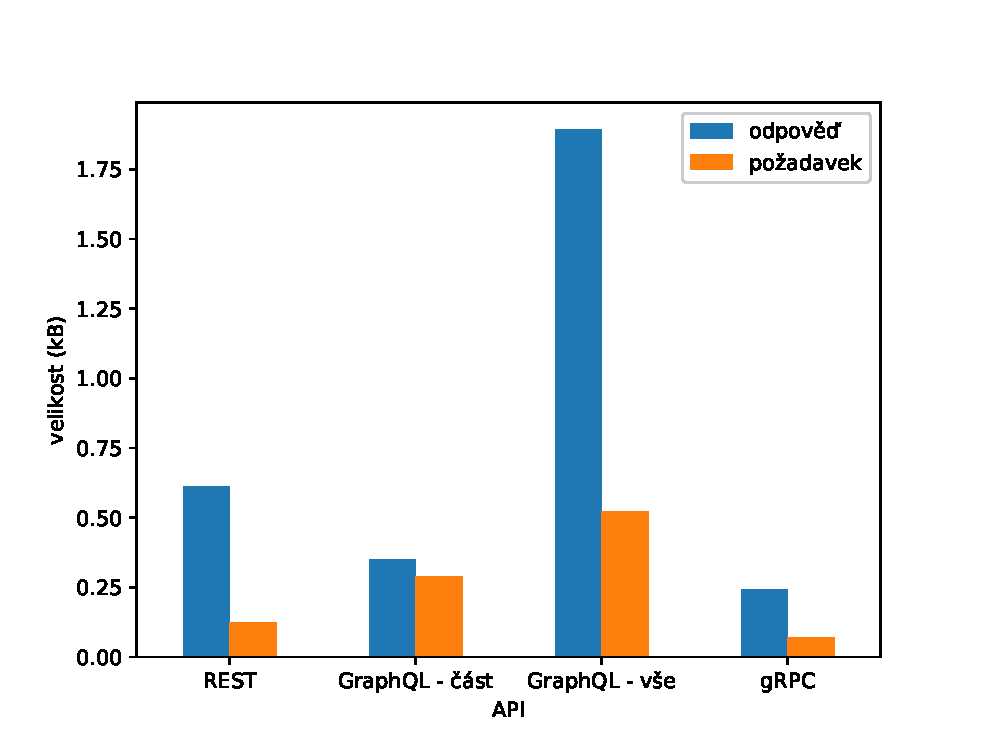
\includegraphics[width=\linewidth]{img/req-size.eps}
  \caption{Detail produktu -- Průměrná velikost odpovědi}
\label{test_get_product_size}
\end{figure}

% \clearpage
\section{Vytvoření nového produktu}
Graf \ref{test_create_product} zobrazuje porovnání výkonu API při vytváření nových produktů. Pro tvorbu nových produktů dokáže zpracovat nejvíce požadavku REST a gRPC API. které podaly téměř stejné výsledky. Výrazně pomalejší pak bylo GraphQL API -- jak verze se zobrazením podmnožiny polí, tak verze se zobrazením všech polí.

\begin{figure}[]
  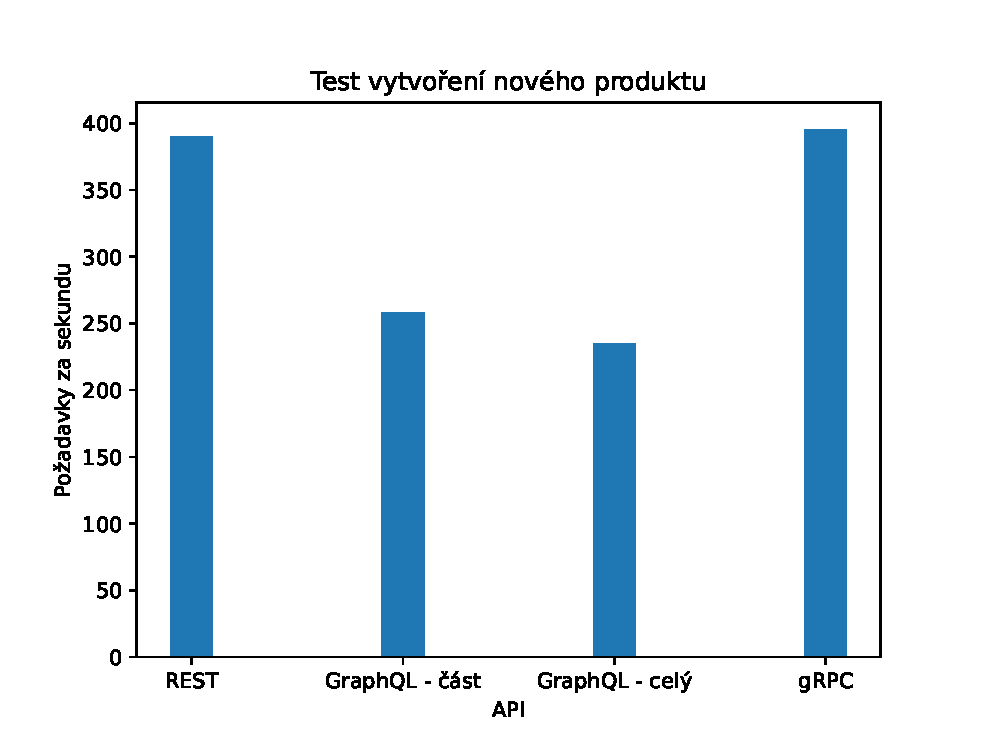
\includegraphics[width=\linewidth]{img/create-product.eps}
  \caption{Vytvoření produktu -- Počet odbavených požadavků za sekundu}
\label{test_create_product}
\end{figure}

Graf \ref{test_create_product_size} pak zobrazuje průměrnou velikost požadavků a odpovědí při tvorbě nových produktů. 

Stejně jako v předchozím testu, gRPC má nejmenší velikost požadavků. Za ním následuje GraphQL zobrazující podmnožinu polí produktu. Následuje REST API a s největší velikostí požadavků GraphQL vracející celý detail produktu.

gRPC má také stále i nejmenší velikost odpovědí. Následuje GraphQL API vracející omezenou podmnožinu polí, poté REST API a následně GraphQL vracející všechna pole produktu.
\begin{figure}[]
  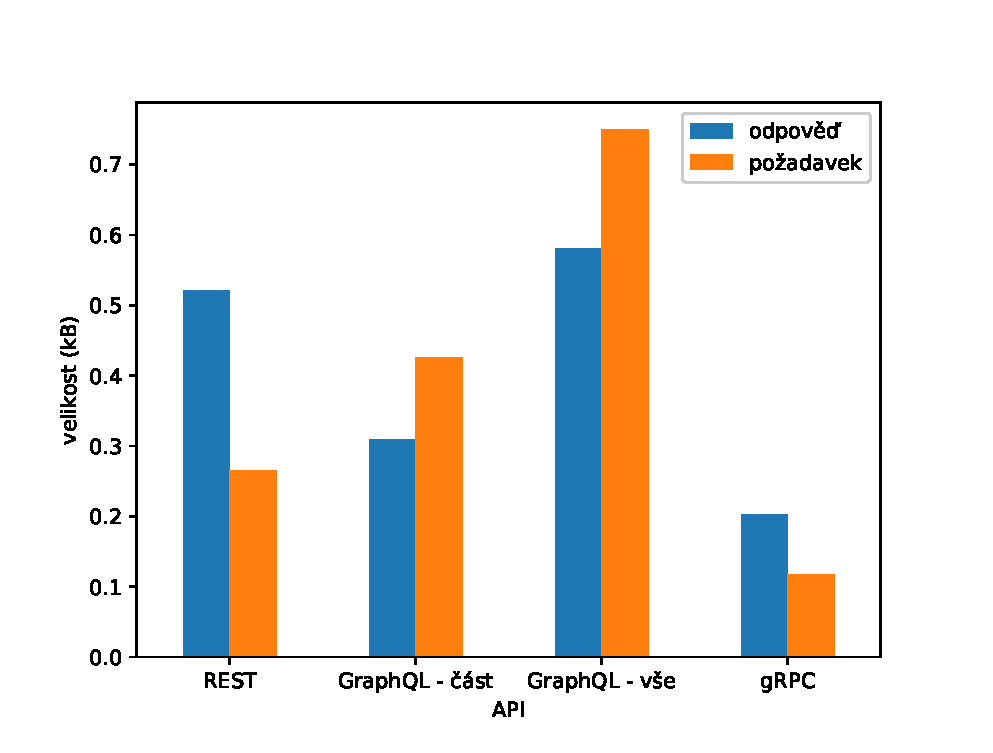
\includegraphics[width=\linewidth]{img/req-size-create.eps}
  \caption{Vytvoření produktu -- Průměrná velikost odpovědi}
\label{test_create_product_size}
\end{figure}


\section{WebSocket, GraphQL subscription a gRPC stream}
Tyto speciální endpointy jsem zkoumal ze dvou pohledů -- maximální počet možných spojení a odezva odpovědi s přibývajícím počtem spojení.

\begin{itemize}
  \item Maximální počet spojení -- pomocí vlastního scriptu jsem testoval následující počty současných spojení --  10, 100, 1000, 10 000, 20 000, 30 000.
  \item Odezva odpovědi -- na serveru jsem nastavil odesílání odpovědi po době 100 milisekund a v klientovi jsem měřil prodlevu mezi jednotlivými odpověďmi. Časová prodleva byla měřena pomocí Node.js knihovny \\* \mintinline{text}{perf_hooks}.
\end{itemize}

\begin{table}[h]
  \begin{tabular}{|l|l|l|l|l|l|l|}
  \hline
  \textbf{implementace \textbackslash spojení} & \textbf{10}     & \textbf{100}    & \textbf{1 000  }& \textbf{10 000}& \textbf{20 000} \\ \hline
  \textbf{REST}                                      & 101 ms & 103 ms & 102 ms & 144 ms & 382 ms   \\ \hline
  \textbf{GraphQL}                                   & 102 ms & 101 ms & 103 ms & 683 ms & N/A      \\ \hline
  \textbf{gRPC}                                      & 100 ms & 100 ms & 101 ms & N/A    & N/A      \\ \hline
  \end{tabular}
  \caption{Test počtu spojení pro REST, GraphQL a gRPC implementace}
\end{table}

\clearpage
\subsubsection*{Počet aktivních spojení}
Nejvíce aktivních spojeních byla schopna obsloužit RESTová implementace pomocí WebSocketů -- 20 000. Dále jsem zkoušel test pro 30 000 spojení, kde jsem ale narazil na limit počítače, na kterém probíhal test, protože už neměl dostatek portů pro tvorbu nových spojení.

Na druhém místě v testu skončila gRPC implementace streamů, která v testu dokázala obsloužit 10 000 spojení. Během testu 20 000 spojení server začal při cca 15 000 aktivních spojení aktivně odmítat nová spojení.

Na posledním místě skončila implementace GraphQL subscriptions. Server dokázal obsloužit 10 000 příchozích spojení. Při testu 20 000 spojení server zamrzl a přestal jakkoli odpovídat.

\subsubsection*{Prodleva mezi posílanými zprávami}
Nejmenší prodlevy dosáhla REST implementace, kdy jako jediná dokázala obsloužit 20 000 spojení s průměrnou prodlevou 382 ms.

GraphQL implementace pak dokázala obsloužit 10 000 spojení s průměrnou odezvou 683 ms. Pro gRPC implementaci nešlo průměrnou prodlevu změřit, protože ačkoli server posílal data, nestíhal a dávkoval několik zpráv dohromady.

\chapter{Závěrečné srovnání}
V této kapitole provedu srovnání technologií REST, GraphQL a gRPC a jejich implementací v jazyce JavaScript. Je potřeba zdůraznit, že některá kritéria jako např. developer experience jsou silně závislá na knihovnách, které jsem pro implementaci API v této práci zvolil.

\section{Srovnávací kritéria}
Abychom mohli tyto technologie mezi sebou porovnat, je nejdříve potřeba stanovit kritéria, podle kterých tyto technologie budeme hodnotit. Popisované technologie porovnám podle následujících kritérií.


\subsection{Oblíbenost}
Oblíbenost dané technologie je velmi důležitým kritériem. Souvisí s ní dostupnost a kvalita dokumentace, rychlost opravy chyb a vývoj nových funkcionalit. Čím více je daná technologie populární mezi vývojáři, je také pravděpodobnější, že v případě nějakého problému s implementací najdeme pomoc právě v nějaké komunitě jako je např. Stack Overlow \cite{stack_overflow}.

Oblíbenost dané technologie se dá kvantifikovat několika způsoby. Poměrně dobrým indikátorem popularity může být například počet hvězd v GitHub repozitáři dané knihovny nebo počet stažení v balíčkovacím systému npm.

Vzhledem k tomu, že tyto technologie nejsou závislé na platformě a v rámci jednotlivých programovacích jazyků existuje mnoho jejich implementací pomocí různých knihoven, je velmi náročné shromáždit data o jejich používání. Rozhodl jsem se proto, že shromáždím nejvíce používané knihovny implementující danou technologii a srovnání provedu nad nimi.

\subsection{Developer experience}
V této části popíšu svoje zkušenosti, které jsem získal při vývoji API pomocí těchto technologií. Přestože se jedná o víceméně subjektivní, věřím že bude přínosem pro každého, kdo přemýšlí o využití některé z těchto technologií.

Práce s dokumentací je nedílnou součástí vývoje a její čitelnost přímo ovlivňuje rychlost s jakou jsme schopni danou knihovnu začít používat nebo jak efektivně vyřešíme problém, na který při vývoji narazíme. Protože tato část je také velmi subjektivní, ke svojí zkušenosti také poskytnu ukázky dokumentaci aby si čtenář mohl udělat svůj názor. 

\subsection{Dokumentace API}
Kvalitní dokumentace API pomáhá ostatní vývojářům pochopit jakými způsoby lze API používat.

\subsection{Verzování API}
Protože většina API se v čase vyvíjí a je potřeba přidávat či měnit funkcionality, je důležité zhodnotit API z pohledu verzování.

\subsection{Výkon}
Potřebujeme-li vybudovat API, které by dokázalo odbavovat velké množství požadavků najednou a co nejrychleji, je výkon nejspíše jedno z hlavních kritérií, které zvažujeme při výběru technologie pro tvorbu API.

V této části porovnám výkon implementovaných API na datech posbíraných během výkonnostního testování z několika pohledů:

\begin{itemize}
    \item Počet odbavených požadavků za sekundu
    \item Velikost odesílaných dat v odpovědi
    \item Počet otevřených spojení WebSocket, GraphQL subscription \\* a gRPC streaming
    \item Prodleva mezi odpověďmi WebSocket, GraphQL subscription a gRPC streaming
\end{itemize}

Musíme však brát v potaz, že výkon serveru může být ovlivněný přístupy do databáze nebo voláním služeb třetích stran.

\section{Srovnání}

\subsection{Oblíbenost}
Jak lze vyčíst z počtu stažení balíčků z npm nebo počtu hvězd jednotlivých frameworků, nejpopulárnější technologií pro tvorbu API je REST, poté následuje GraphQL a za ním gRPC.

Musíme však brát v potaz, že počet stažení je ovlivněn např. automatickými testy, které toto číslo zvětšují.

\subsubsection*{REST}
\begin{table}[h]
  \begin{tabular}{|l|l|l|}
  \hline
  \textbf{balíček}      & \textbf{stažení za týden}     & \textbf{GitHub hvězdy} \\ \hline
  \textbf{express}      & 23 mil.                       & 56 748                 \\ \hline
  \textbf{@nestjs/core} & 1,3 mil.                      & 45 994                 \\ \hline
  \textbf{koa}          & 1,1 mil.                      & 32 539                 \\ \hline
  \end{tabular}
  \caption{REST frameworky - počty stažení a hvězd \cite{rest_trends}}
\end{table}

\subsubsection*{GraphQL}
\begin{table}[h]
  \begin{tabular}{|l|l|l|}
  \hline
  \textbf{balíček}                                 & \textbf{stažení za týden}                           & \textbf{GitHub hvězdy} \\ \hline
  \textbf{apollo-server-core}                      & 2 mil.                                              & 12 475                 \\ \hline
  \textbf{express-graphql}                         & 0,6 mil.                                            & 6 182                  \\ \hline
  \textbf{graphql-yoga}                            & 21 tis.                                             & 6 782                  \\ \hline
  \end{tabular}
  \caption{GraphQL frameworky -- počty stažení a hvězd \cite{graphql_trends}}
\end{table}

\subsubsection*{gRPC}
\begin{table}[h]
  \begin{tabular}{|l|l|l|}
  \hline
  \textbf{balíček}                                 & \textbf{stažení za týden}                           & \textbf{GitHub hvězdy} \\ \hline
  \textbf{@grpc/grpc-js}                           & 3,2 mil.                                            & 3 386                  \\ \hline
  \textbf{mali}                                    & 40 tis.                                             & 794                    \\ \hline
  \textbf{protocat}                                & 359                                                 & 42                     \\ \hline
  \end{tabular}
  \caption{gRPC frameworky -- počty stažení a hvězd \cite{grpc_trends}}
\end{table}

\subsection{Developer Experience}
\subsubsection*{REST}
Implementace RESTového API s použitím Expressu je určitě nejjednodušší a nejrychlejší ze všech tří způsobů. K prvotnímu nastavení a spuštění serveru stačí napsat pár řádek kódu a nic nebrání pokračování na implementaci.
Nespornou výhodou Expressu je jeho popularita. Pokud by nám nestačila oficiální dokumentace, existuje velké množství návodů nebo odpovědí na Stack Overflow, které nám mohou pomoci.

\subsubsection*{GraphQL}
S GraphQL jsem se setkal poprvé během této práce a mile mě překvapilo. Překvapila mě jednoduchost implementace -- není totiž třeba implementovat výběr jednotlivých polí, které si uživatel specifikuje při dotazu, stačí pouze v Resolveru vrátit objekt správného typu a o projekci polí se postará knihovna sama. Samotná implementace GraphQL API se tak moc obtížností nelišila od RESTu. 

Dobře se mi pracovalo s knihovnou \mintinline{text}{type-graphql}\cite{typegraphql_doc}, který díky dekorátorům dělá kód dobře čitelný a strukturovaný. Tato knihovna také obsahuje často používané funkcionality -- např. ověřování uživatelů. Jako jedna z největších výhod při vývoji se mi jeví automatické generování GraphQL schématu při spouštění serveru -- udržování dokumentace API je věc, na kterou spousta vývojářů často zapomíná. Jako nevýhodu však můžu zmínit strmou učící křivku nebo složité psaní dotazů při testech, kdy je při dotazování nutné vypisovat v dotazech všechna dostupná pole.

\subsubsection*{gRPC}
Inicializace projektu pro gRPC API byla ze všech nejnáročnější. Je potřeba navrhnout strukturu API do protocol buffer souborů, zkompilovat je a poté správně naimportovat a vytvořit server. Jakmile je ale vše připraveno, vývoj probíhá vcelku bez problémů.

S frameworkem pro gRPC server ProtoCat se mi pracovalo velmi dobře a oproti referenční implementaci gRPC šetří spoustu práce. Přes vcelku dobrou zkušenost zmíním dvě nevýhody, se kterými jsem se při vývoji setkal. První je nutnost serializace výsledků gRPC volání do zpráv, kdy je nutné zavolat metodu pro serializaci pro každý jeden atribut, který se ve zprávě vyskytuje. Co však považuji jako zásadní nevýhodu je nedostatek dokumentace pro tento framework, kdy jsem chvílemi musel spoléhat na procházení zdrojových kódů frameworku nebo na našeptávač ve vývojovém prostředí, který naštěstí díky TypeScriptu fungoval dobře.

Ještě musím jako výhodu zmínit jednoduchou implementaci streamů. Díky tomu, že gRPC funguje na \mintinline{text}{HTTP/2}, pro implementaci streamů není potřeba přidávat žádný další server, jak to bylo potřeba pro implementaci WebSocketů. Stačí tak pouze v protocol bufferu označit typ metody klíčovým slovem \mintinline{text}{stream}.


\subsection{Dokumentace API}
\subsubsection*{REST}
Pro dokumentaci REST API existují dva způsoby, jak přistupovat ke tvorbě API jeho dokumentace: design first a program first.%todo% 
V prvním případě nejdříve navrhujeme samotné API např. ve specifikaci OpenAPI a poté využijeme nějaký program třetí strany k vygenerování kostry API nebo typů pro TypeScript.

Ve druhém případě API nejdříve naprogramujeme a poté pomocí knihovny vygenerujeme samotnou dokumentaci, také např. ve formátu OpenAPI. Tento přístup má hlavní výhodu v tom, že dokumentaci nemusíme věnovat takovou práci údržbě dokumentace. Na druhou stranu může být práce programátora snazší, pokud už má návrh připravený a programuje podle něj.

\subsubsection*{GraphQL}
GraphQL je na tom o něco lépe co se týče dokumentace. Pro prozkoumání možností API si můžeme buď zobrazit GraphQL schéma, kde je celá struktura API definována, nebo můžeme využít vlastnosti introspekce a aplikační rozhraní si pomocí GraphQL dotazů vyzkoušet.

Samozřejmě je možné využít nějaký nástroj k zobrazení a práci s API. Při programování GraphQL API se mi osvědčil nástroj GraphQL Playground \cite{apollo_playground}. 
Jedná se o nástroj vyvinutý Prismou a založený na GraphiQL, který umožňuje v prohlížeči interaktivně provolávat GraphQL API. Mezi jeho hlavní funkcionality patří automatické doplňování textu a zvýrazňování chyb nebo testování GraphQL subscriptions. Zároveň je velmi jednoduché tento nástroj začít používat, stačí ho aktivovat jako plugin při inicializaci serveru.


\subsubsection*{gRPC}
Stejně jako GraphQL, tak i gRPC nutí vývojáře udržovat kontrakt specifikující chování API.
Protože při tvorbě gRPC API je potřeba vytvořit definici služeb a metod pomocí \mintinline{text}{.proto} souborů, máme tak určitou formu dokumentace API přímo dostupnou.

Kromě samotného čtení můžeme využít nástrojů třetích stran, které je možné použít jak k prozkoumávání možností API, tak zároveň k jeho testování. Mohu například zmínit nástroj BloomRPC \cite{bloomrpc}, který jsem používal k testování API při implementaci. Tento nástroj podporuje všechny typy gRPC metod od \mintinline{text}{unary call} po \mintinline{text}{bidirectional streaming}. Díky specifikaci typů zpráv v protocol bufferu, tento nástroj připraví dotazy na jednotlivé metody s vyplněnými výchozími hodnotami. Na rozdíl od GraphQL Playground, tato aplikace není dostupná jako plugin serveru, ale je potřeba si ji doinstalovat. Poté stačí importovat si příslušné \mintinline{text}{.proto} soubory, nakonfigurovat k jakému serveru se chceme připojit a začít testovat API.

\subsubsection*{Zhodnocení}
Z hlediska dokumentace API mi jako nejlepší vycházejí GraphQL a gRPC. Obě technologie z principu nutí udržovat vývojáře nějaký způsob dokumentace API, s tím že GraphQL je na tom ještě o něco lépe díky introspekci.

REST z tohoto úhlu pohledu vychází na posledním místě, ale to neznamená, že by na tom byl špatně. Je jen nutno počítat s tím, že je potřeba věnovat čas a rozmyslet si, jak budeme dokumentaci API tvořit a udržovat.

\subsection{Verzování API}
Z pohledu verzování je na tom nejlépe GraphQL. Pokud nebudeme dělat breaking-changes, ale jen přidávat nové funkcionality a pole, a ty zastaralá necháme být bez porušení zpětné kompatibility, můžeme se verzování úplně vyhnout. Díky možnosti specifikace tvaru dotazů můžeme totiž tyto zastaralá pole úplně ignorovat a vyhneme se tak nabobtnávání odpovědí serveru.

U REST API se verzování v některých případech nevyhneme, ale máme pořád větší svobodu než u gRPC.

Úplně nejhůře je na tom z pohledu verzování gRPC, je totiž nutné aktualizovat klienty skoro při každé změně Protocol Bufferu, výjimkou může být např. přidání úplně nové služby, kterou stávající klienti nebudou používat.

\subsection{Výkon}

\subsubsection*{Počet odbavených požadavků za sekundu}
Při testu zobrazování detailu produktu byly všechny servery srovnatelně schopné odbavovat požadavky. Při vytváření nových produktů pak znatelně zaostávalo GraphQL, může to však být závislé na implementaci a je tak těžké zhodnotit zda jedna technologie je rychlejší či ne.
\subsubsection*{Velikost odesílaných dat v odpovědi}
Při odesílání požadavků pro zobrazující celé odpovědi, nejmenší odpovědi mělo gRPC. Pokud by však byla relevantní jen nějaká podmnožin polí, GraphQL může mít menší velikost odpovědí.
\subsubsection*{Prodleva zpráv při použití WebSocket, GraphQL subscription a gRPC streaming}
Nejlépe zatížení zvládal WebSocket, který pro 10 000 aktivních spojeních odesílal odpovědi s prodlevou 144ms, GraphQL s prodlevou 683ms. Pro gRPC pak prodleva nebyla měřitelná, protože server nestíhal a odesílal odpovědi po dávkách.
\subsubsection*{Počet otevřených spojení HTTP WebSocket, GraphQL subscription a gRPC streaming}
Největší počet aktivních spojení zvládl obsloužit WebSocket. gRPC zvládl obsloužit přibližně 15 000 spojení a další pak už odmítal. GraphQL server zvládl obsloužit 10 000 subscriptions, ale při větším počtu přestal úplně reagovat a zamrzl.

\subsubsection*{Zhodnocení}
Na základě výkonnostního testování je těžké vybrat technologii, která by byla jasným vítězem, protože velmi záleží na volbě a implementaci použitého \\*frameworku. Pro nejmenší zatížení sítě je možné zvolit gRPC, pokud by však byl kladen na specifikaci tvaru odpovědi klientem, bylo by vhodné použít GraphQL.

\begin{conclusion}
Cílem práce bylo představení tří technologií pro tvorbu API -- REST, GraphQL a gRPC, implementace shodných API v Node.js pomocí každé technologie a následné porovnání z hlediska výkonu, DX, dokumentace API nebo verzování.

V kapitole \textit{Analýza} jsou představeny principy, na kterých tyto technologie fungují. Dále je zde také představen jazyk TypeScript, ve kterém byly ukázky API implementovány, společně s prostředím Node.js.

V kapitole \textit{Dostupné technologie} jsem zkoumal dostupné knihovny pro implementaci aplikačních rozhraní a pro každý typ API jsem jednu z knihoven vybral pro ukázkovou implementaci.

Návrhu ukázkového API pro e-shop, na kterém byly demonstrovány implementace a rozdíly mezi technologiemi jsem se věnoval v kapitole \textit{Návrh}.

Různé aspekty implementace a testů jednotlivých API jsou popsány v kapitole \textit{Implementace}. Tyto implementace jsem poté podrobil zátěžovým testům a provedl zhodnocení podle rychlosti, dokumentace a vývojářské zkušenosti.

Rychlostně mezi technologiemi nebyly žádné zásadní rozdíly, jen při potřebě streamování nějaké sekvence dat bych určitě nevolil GraphQL subscriptions. Ta jsou vhodnější pro ne tak časté aktualizace dat.

Z porovnání jednotlivých technologií nevyšel jasný vítěz, záleží na konkrétních požadavcích a způsobu, jakým bude API použito. Pro implementaci obecného API, které bude veřejné bych zvolil REST. Použití GraphQL mi dává smysl v případě, kdy potřebujeme číst velké množství dat, ze kterých jsou relevantní jen nějaké části. gRPC bych naopak volil pro neveřejná API (kvůli nutnosti udržování Protocol Buffer specifikace  a nutnosti HTTP/2) pro komunikaci mezi interními komponentami nebo podpoře streamů.

\end{conclusion}

\bibliographystyle{csn690}
\bibliography{mybibliographyfile}

\appendix

\chapter{Seznam použitých zkratek}
% \printglossaries
\begin{description}
	\item[API] Application programming interface
	\item[CPU] Central processing unit
	\item[DX] Developer experience
	\item[GUI] Graphic user interface
	\item[HTTP] Hypertext Transfer Protocol
	\item[IDE] Integrated development environment
	\item[JSON] JavaScript Object Notation
	\item[JWT] JSON Web token
	\item[NPM] Node Package Manager
	\item[ORM] Object-relational mapping
	\item[REST] Representational State Transfer
	\item[RPC] Remote procedure call
	\item[SQL] Structured Query Language
	\item[URI] Uniform Resource Identifier
	\item[URL] Uniform Resource Locator  
\end{description} 

\chapter{Obsah přiloženého CD}

\begin{figure}
	\dirtree{%
		.1 readme.txt\DTcomment{stručný popis obsahu CD}.
		.1 src.
		.2 shop-graphql\DTcomment{GraphQL implementace}.
    .2 shop-grpc\DTcomment{gRPC implementace}.
    .2 shop-rest\DTcomment{REST implementace}.
    .2 test\DTcomment{implementace zátěžových testů}.
		.2 text\DTcomment{zdrojová forma práce ve formátu \LaTeX{}}.
		.1 text\DTcomment{text práce}.
		.2 DP\_Bunata\_Tomas\_2022.pdf\DTcomment{text práce ve formátu PDF}.
	}
\end{figure}

\end{document}
